\documentclass[12pt,a4paper,oneside]{article}
\usepackage[QX]{polski}
\usepackage[T1]{fontenc}
\usepackage[utf8]{inputenc}
\usepackage{latexsym}
\usepackage{tgpagella}
\usepackage{lmodern}
\usepackage{amsmath,amsthm,amsfonts,amssymb,alltt}
\usepackage{epsfig}
\usepackage{pdflscape}
\usepackage{caption}
\usepackage{indentfirst}
\usepackage{float}
%\usepackage{showkeys}
\bibliographystyle{plabbrv}


\usepackage{color}
\usepackage[polish]{babel}
\usepackage{datetime2}
\usepackage[x11names,dvipsnames,table]{xcolor}
\usepackage{hyperref}
\hypersetup{
pdfauthor={Roman Czapla, Olaf Bar},
colorlinks=True,
linkcolor=darkgray,  % color of internal links (change box color with linkbordercolor)
citecolor=BrickRed,  % color of links to bibliography
filecolor=Magenta,   % color of file links
urlcolor=BlueViolet}	%%pdfpagemode=FullScreen}

% diagramy, grafy itp.
\usepackage{tikz}
\usetikzlibrary{positioning}
\usetikzlibrary{arrows}
\usetikzlibrary{arrows.meta}
\usetikzlibrary{chains,fit,shapes,calc}
\tikzset{main node/.style={circle,fill=blue!20,draw,minimum size=1cm,inner sep=0pt}}

% algorytmy
\usepackage[linesnumbered,lined,commentsnumbered]{algorithm2e}
\SetKwFor{ForEach}{for each}{do}{end for}%
\SetKwFor{ForAll}{for all}{do}{end for}%
\newenvironment{myalgorithm}
{\rule{\textwidth}{0.5mm}\\\SetAlCapSty{}\SetAlgoNoEnd\SetAlgoNoLine\begin{algorithm}}{\end{algorithm}\rule{\textwidth}{0.5mm}}


%---------------------
\overfullrule=2mm
\pagestyle{plain}
\textwidth=15cm \textheight=685pt \topmargin=-25pt \linespread{1.3} 
\setlength{\parskip}{0pt}
\setlength\arraycolsep{2pt}
\oddsidemargin =0.9cm
\evensidemargin =-0.1cm

\captionsetup{width=.95\linewidth, justification=centering}
%---------------------




\newtheorem{tw}{Twierdzenie}[section]
\newtheorem{lem}[tw]{Lemat}
\newtheorem{co}[tw]{Wniosek}
\newtheorem{prop}[tw]{Stwierdzenie}
\theoremstyle{definition}
\newtheorem{ex}{Przykład}
\newtheorem{re}[tw]{Uwaga}
\newtheorem{de}{Definicja}[section]



\newcommand{\bC}{{\mathbb C}}
\newcommand{\bR}{{\mathbb R}}
\newcommand{\bZ}{{\mathbb Z}}
\newcommand{\bQ}{{\mathbb Q}}
\newcommand{\bN}{{\mathbb N}}
\newcommand{\captionT}[1]{\caption{\textsc{\footnotesize{#1}}}}
\renewcommand\figurename{Rys.}

\numberwithin{equation}{section}
\renewcommand{\thefootnote}{\arabic{footnote})}
%\renewcommand{\thefootnote}{\alph{footnote})}



\begin{document}

% --------------------------------------------
% Strona tytułowa
% --------------------------------------------

\thispagestyle{empty}
\begin{titlepage}
\begin{center}\Large
Uniwersytet Komisji Edukacji Narodowej w Krakowie\\
\large
Instytut Bezpieczeństwa i Informatyki\\
\vskip 10pt
\end{center}
\begin{center}
\centering 
\includegraphics[width=1.0\columnwidth]{images/logo.png}
\end{center}

\begin{center}
 {\bf \fontsize{14pt}{14pt}\selectfont PROJEKT INŻYNIERSKI \\ RAPORT Z REALIZACJI PROJEKTU\\
 }
 {\fontsize{12pt}{12pt} raport z okres: 20.10.2024 - 20.01.2025}
\end{center}
\vskip 5pt
\begin{center}
 {\bf \fontsize{12pt}{22pt}\selectfont System rekomendacji produktów. Tworzenie algorytmu rekomendacyjnego na
 podstawie preferencji użytkowników – aplikacja przeglądarkowa}
\end{center}

\begin{center}
 {\fontsize{12pt}{12pt}\selectfont wykonany przez: }
\end{center}
\begin{center}
 {\bf\fontsize{16pt}{16pt}\selectfont Krzysztof Bielkiewicz}\\
 {\fontsize{12pt}{12pt}\selectfont Nr albumu: 156791 \\\&\\}
 {\bf\fontsize{16pt}{16pt}\selectfont Maciej Fabef}\\
 {\fontsize{12pt}{12pt}\selectfont Nr albumu: 156750\\\&\\}
 {\bf\fontsize{16pt}{16pt}\selectfont Grzegorz Golonka }\\
 {\fontsize{12pt}{12pt}\selectfont Nr albumu: 156742}
\end{center}
\begin{center}
 {\fontsize{12pt}{12pt}\selectfont pod opieką:}\\
 {\bf\fontsize{12pt}{12pt}\selectfont dr hab. inż. Mateusz Muchacki, prof. UKEN}
\end{center}

%\mbox{}
\vspace*{\fill}
%\vskip 50pt
\begin{center}
\large
Kraków \the\year\\
(ostatnia aktualizacja: \DTMcurrenttime,\;\today)
\end{center}
\end{titlepage}
\setcounter{page}{0} 
\newpage\null\thispagestyle{empty}
%\setcounter{page}{0} 
%\newpage
%\thispagestyle{empty}

\tableofcontents


\newpage

\section{Informacja na temat postępów prac nad projektem}

\subsection{Zespół projektowy}
\textit{Lista osób tworzących zespół projektowy wraz z danymi kontaktowi (e-mail).}
    \paragraph{Grzegorz Golonka}
    \begin{itemize}
        \item E-mail: grzegorz.golonka@student.up.krakow.pl
    \end{itemize}
    \paragraph{Krzysztof Bielkiewicz}
    \begin{itemize}
        \item E-mail:  krzysztof.bielkiewicz@student.up.krakow.pl
    \end{itemize}
    \paragraph{Maciej Faber}
    \begin{itemize}
        \item E-mail: maciej.faber@student.up.krakow.pl
    \end{itemize}

\subsection{Zrealizowane zadania}
\textit{Lista zrealizowanych prac z podziałem na członków zespołu projektowego.}
\paragraph{Krzysztof Bielkiewicz}
\begin{itemize}
    \item Zadanie 1. Stworzenie nagłówka dla aplikacji (\hyperref[1.3.1]{sekcja 1.3.1})
    \item Zadanie 2. Stworzenie strony startowej (\hyperref[1.3.2]{sekcja 1.3.2})
    \item Zadanie 3. Opcja wyszukiwania po słowach kluczowych (\hyperref[1.3.3]{sekcja 1.3.3})
    \item Zadanie 4. Opcja wyszukiwania po kategoriach (\hyperref[1.3.4]{sekcja 1.3.4})
    \item Zadanie 5. Stworzenie strony z ulubionymi produktami (\hyperref[1.3.5]{sekcja 1.3.5})
    \item Zadanie 6. Stworzenie strony profilu z opcją edycji (\hyperref[1.3.6]{sekcja 1.3.6})
    \item Zadanie 7. Oprawa graficzna dla strony dodania adresu dostawy (\hyperref[1.3.7]{sekcja 1.3.7})
    \item Zadanie 8. Oprawa graficzna koszyka (\hyperref[1.3.8]{sekcja 1.3.8})
    \item Zadanie 9. Oprawa graficzna wyboru adresu dostawy (\hyperref[1.3.9]{sekcja 1.3.9})
    \item Zadanie 10. Oprawa graficzna dla metod płatności (\hyperref[1.3.10]{sekcja 1.3.10})
    \item Zadanie 11. Oprawa graficzna szczegółów zamówienia (\hyperref[1.3.11]{sekcja 1.3.11})
    \item Zadanie 12. Oprawa graficzna dla listy zamówień (\hyperref[1.3.12]{sekcja 1.3.12})
    \item Zadanie 13. Wyświetlanie produktów z bazy danych (\hyperref[1.3.13]{sekcja 1.3.13})
    \item Zadanie 14. Funckja dodawania produktów do ulubionych (\hyperref[1.3.14]{sekcja 1.3.14})
    \item Zadanie 15. Paginacja produktów na stronach (\hyperref[1.3.15]{sekcja 1.3.15})
    \item Zadanie 16. Oprawa graficzna szczegółów produktu (\hyperref[1.3.16]{sekcja 1.3.16})
    \item Zadanie 17. Custom errory i oprawa graficzna rejestracji (\hyperref[1.3.17]{sekcja 1.3.17})
    \item Zadanie 18. Custom errory i oprawa graficzna loginu (\hyperref[1.3.18]{sekcja 1.3.18})
\end{itemize}
\paragraph{Grzegorz Golonka}
\begin{itemize}
    \item Zadanie nr 1. Utworzenie pliku README.md                          (\ref{section:1.3.19})
    \item zadanie nr 2. Utworzenie modeli bazodanowych                      (\ref{section:1.3.20})
    \item Zadanie nr 3. Dodanie skryptów do inicjalizacji projektu          (\ref{section:1.3.21})
    \item Zadanie nr 4. Stworzenie seeda produktów i kategorii              (\ref{section:1.3.22})
    \item Zadanie nr 5. Formularze do modelów bazodanowych                  (\ref{section:1.3.23})
    \item Zadanie nr 6. Obsługa widoków adresu i listy adresów użytkownika  (\ref{section:1.3.24})
    \item Zadanie nr 7. Obsługa widoków metody płatności i kodu Blik        (\ref{section:1.3.25})
    \item Zadanie nr 8. Weryfikacja danych przy składaniu zamówienia               (\ref{section:1.3.26})
    \item Zadanie nr 9. Tworzenie zamówienia i wysyłanie powiadomień               (\ref{section:1.3.27})
    \item Zadanie nr 10. Implementacja widoku szczegółów zamówienia              (\ref{section:1.3.28})
    \item Zadanie nr 11. Automatyczna aktualizacja statusu zamówienia              (\ref{section:1.3.29})
    \item Zadanie nr 12. Przygotowanie do oceniania produktów w zamówieniu             (\ref{section:1.3.30})
    \item Zadanie nr 13. Automatyczne tworzenie konwersacji przy zamówieniu             (\ref{section:1.3.31})
    \item Zadanie nr 14. Widok listy wiadomości i konwersacji              (\ref{section:1.3.32})
    \item Zadanie nr 15. Obsługa ładowania wiadomości              (\ref{section:1.3.33})
    \item Zadanie nr 16. Utworzenie systemu oceniania produktów             (\ref{section:1.3.34})
    \item Zadanie nr 17. Integracja systemu ocen z widokiem produktu            (\ref{section:1.3.35})
    \item Zadanie nr 18.  Dynamiczna obsługa ocen i ich edycji             (\ref{section:1.3.36})

\end{itemize}
\paragraph{Maciej Faber}
\begin{itemize}
    \item Zadanie nr 1. Obsługa rejestracji (\ref{section:1.3.37})
    \item Zadanie nr 2. Logowanie przy użyciu adresu e-mail (\ref{section:1.3.38})
    \item Zadanie nr 3. Stworzenie modeli obsługujących koszyk (\ref{section:1.3.39})
    \item Zadanie nr 4. Widoki obsługujące zarządzanie koszykiem (\ref{section:1.3.40})
    \item Zadanie nr 5. Konfiguracja i obsługa wysyłania e-maili za pomocą Gmail API (\ref{section:1.3.41})
    \item Zadanie nr 6. Import danych z pliku JSON do bazy danych aplikacji (\ref{section:1.3.42})
    \item Zadanie nr 7. Import zdjęć produktów z bazy danych (\ref{section:1.3.43})
    \item Zadanie nr 8. Sortowanie wyświetlanych produktów (\ref{section:1.3.44})
    \item Zadanie nr 9. Filtrowanie wyświetlanych produktów (\ref{section:1.3.45})
    \item Zadanie nr 10. Dodanie kodu HTML obsługującego sortowanie w szablonach (\ref{section:1.3.46})
    \item Zadanie nr 11. Model \texttt{UserProductVisibility} i logowanie wyświetlanych produktów (\ref{section:1.3.47})
    \item Zadanie nr 12. Model \texttt{UserCategoryVisibility} i logowanie wyświetlanych kategorii (\ref{section:1.3.48})
    \item Zadanie nr 13. Model \texttt{UserQueryLog} i logowanie zapytań użytkownika (\ref{section:1.3.49})
    \item Zadanie nr 14. Modele używane w algorytmie rekomendacyjnym (\ref{section:1.3.50})
    \item Zadanie nr 15. Utworzenie algorytmu rekomendacyjnego (\ref{section:1.3.51})
    \item Zadanie nr 16. Aktualizacja algorytmu rekomendacyjnego o skuteczność propozycji (\ref{section:1.3.52})
    \item Zadanie nr 17. Algorytm rekomendacyjny dla sesji (\ref{section:1.3.53})
    \item Zadanie nr 18. Program do skalowania zdjęć produktów (\ref{section:1.3.54})
\end{itemize}

\subsection {Opis zrealizowanych prac}
\subsubsection{Krzysztof Bielkiewicz: Stworzenie nagłówka dla aplikacji}
\label{1.3.1}
\textit{Responsywny nagłówek dla całej aplikacji, zawierający:}
\begin{itemize}
    \item Nazwe aplikacji, funkcje wyszukiwania
    \item Przycisk z wyborem kategorii i przekierowania do produktów z wybranej kategorii
    \item Przyciski przekierowania do strony z Ulubione i Koszyka
    \item Przycisk Profile pokazujący przyciski przekierowujące do:
        \begin{itemize}
            \item Edycji profilu, Dodania adresu
            \item Wiadomości, Szczegółów zamówienia
            \item Wylogowania
        \end{itemize}
\end{itemize}

\begin{figure}[H]
    \centering
    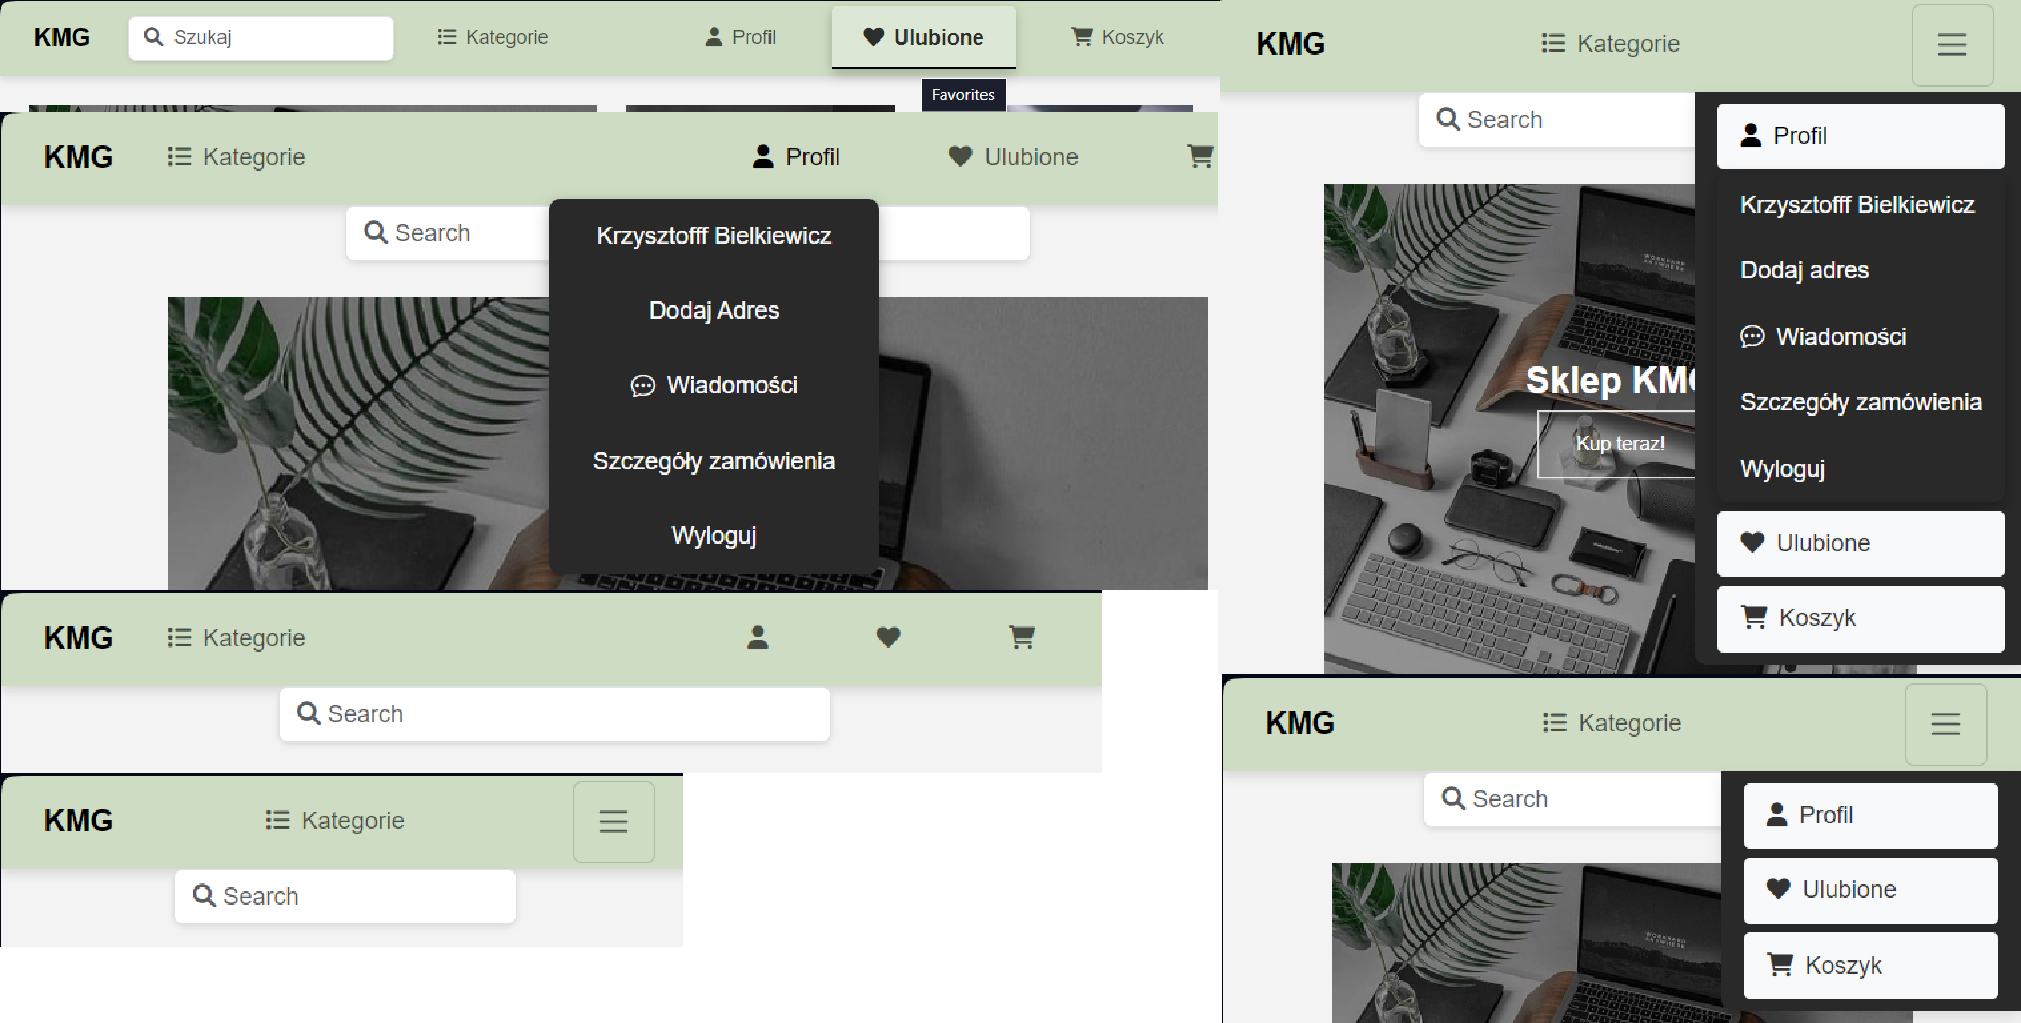
\includegraphics[width=0.9\columnwidth]{images/krzysztofBImages/header.png}
    \caption{Nagłówek z przyciskami}
    \emph{Źródło: opracowanie własne.}
\end{figure}

\begin{figure}[H]
    \centering
    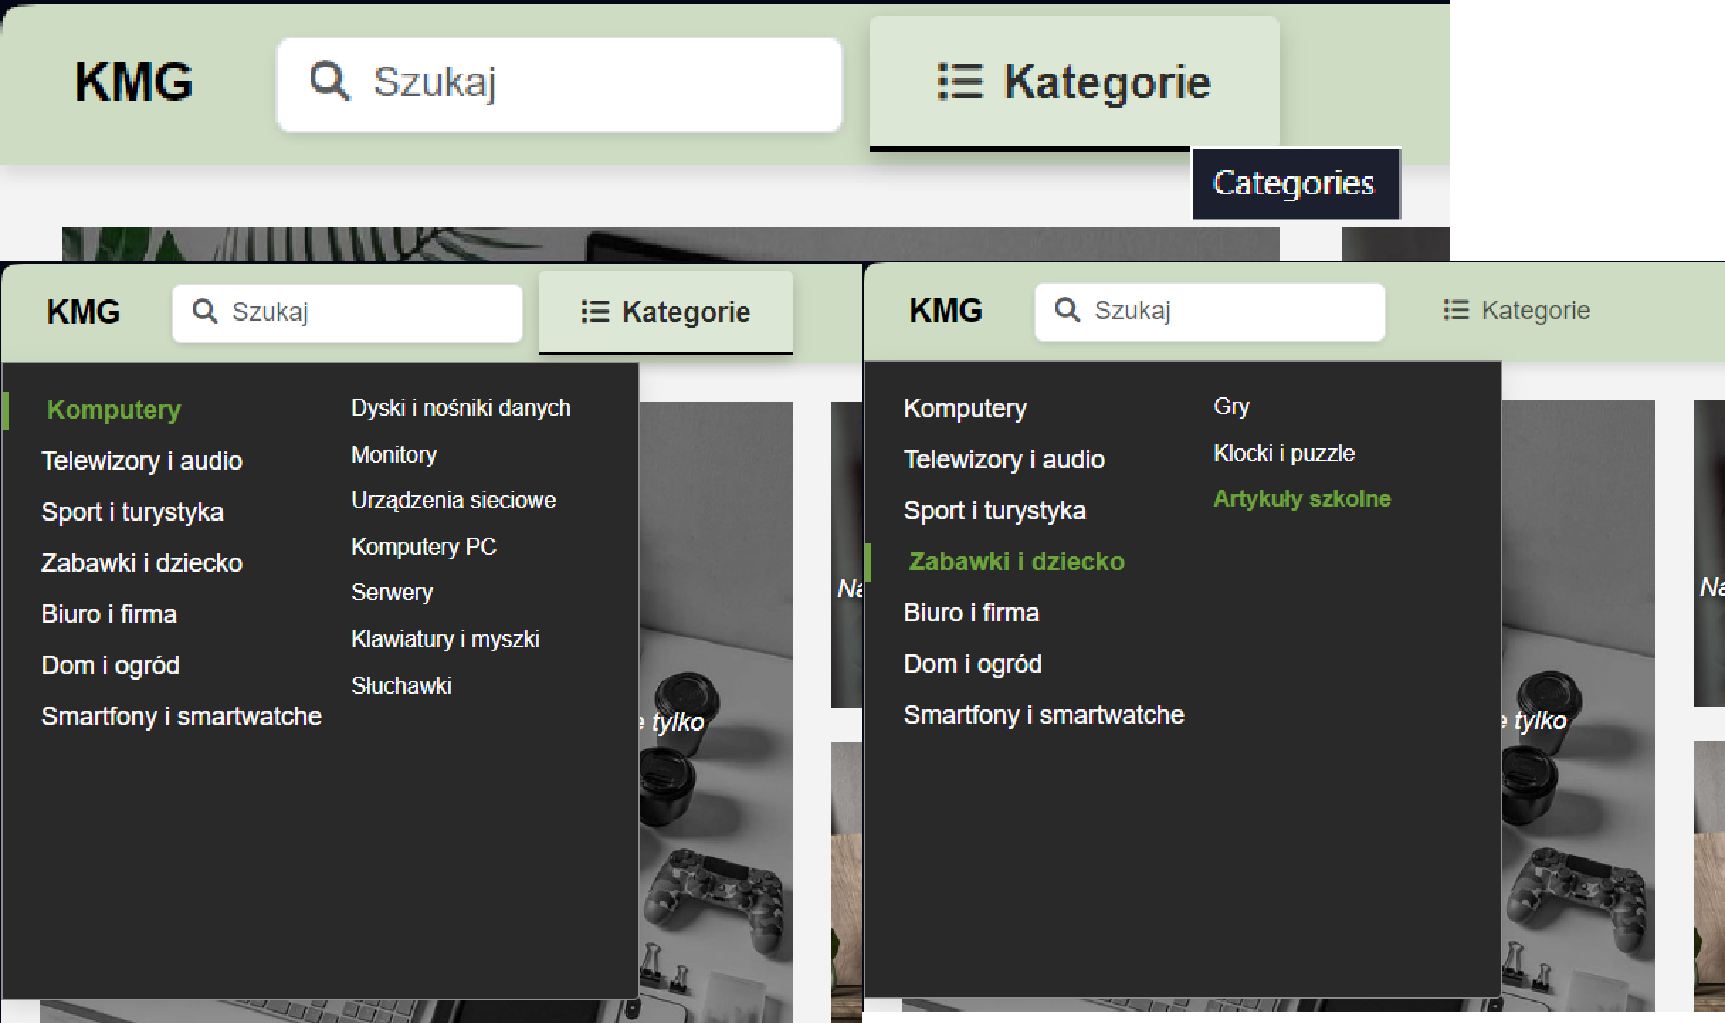
\includegraphics[width=0.9\columnwidth]{images/krzysztofBImages/header-categories.png}
    \caption{Wybór kategorii w nagłówku}
    \emph{Źródło: opracowanie własne.}
    \label{header-categories}
\end{figure}


\subsubsection{Krzysztof Bielkiewicz: Stworzenie strony startowej}
\label{1.3.2}
\textit{Responsywna strona startowa zawierająca:}
    \begin{itemize}
        \item Główny baner z przekierowaniami do poszczególnych kategorii
        \item Interaktywny slider wyświetlający polecane produkty oraz drugi co wyświetla polubione produkty
        \item Stopka
    \end{itemize}

    \begin{figure}[H]
        \centering
        
\includegraphics[width=0.8\columnwidth]{images/krzysztofBImages/main-banner.png}
        \caption{Główny banner}
        \emph{Źródło: opracowanie własne.}
    \end{figure}

    \begin{figure}[H]
        \centering
        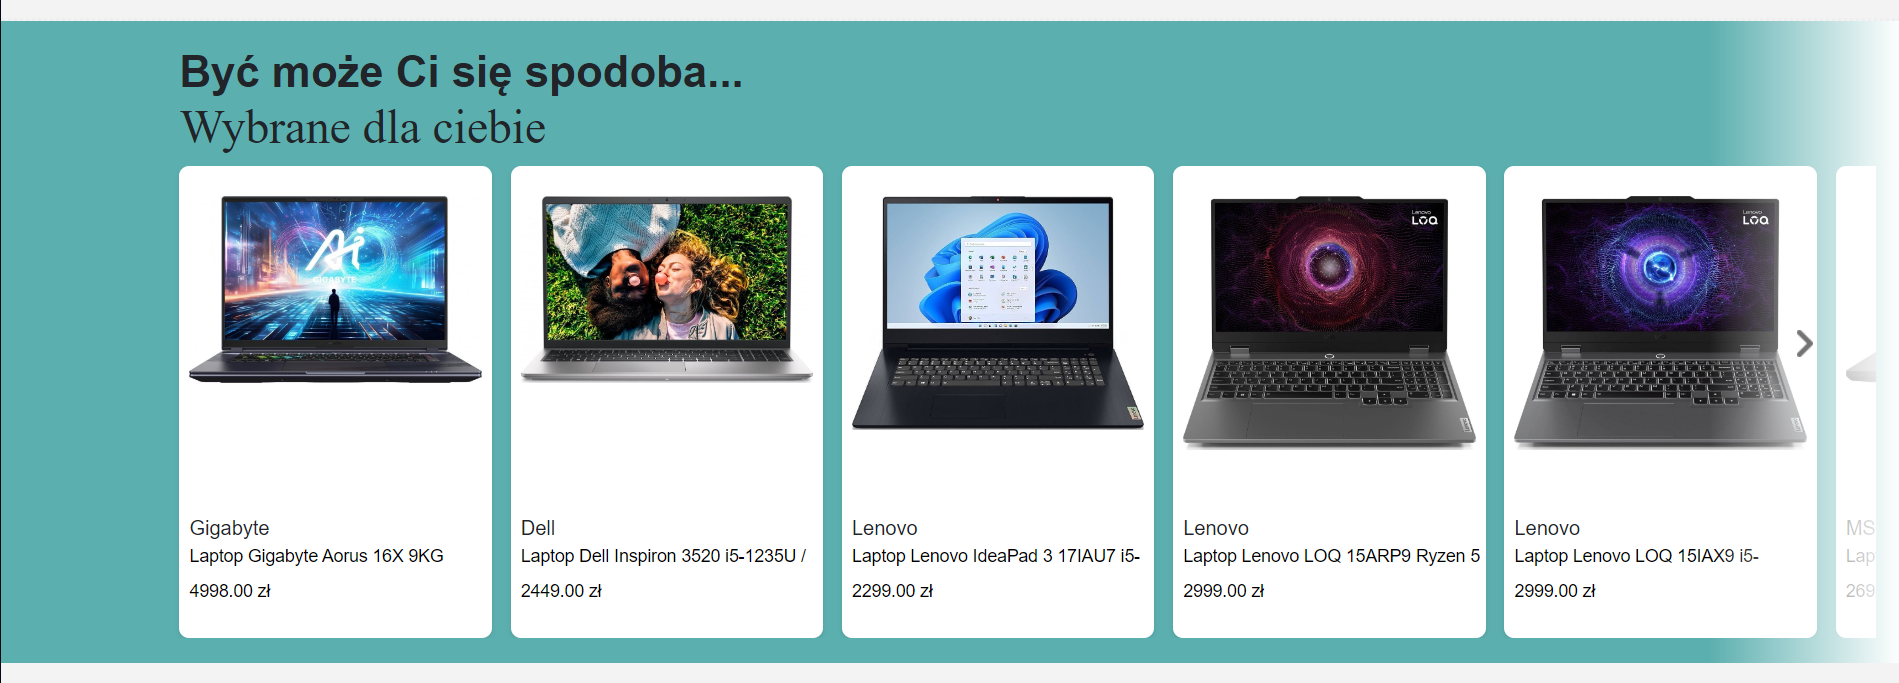
\includegraphics[width=0.7\columnwidth]{images/krzysztofBImages/slider-polecane.png}
        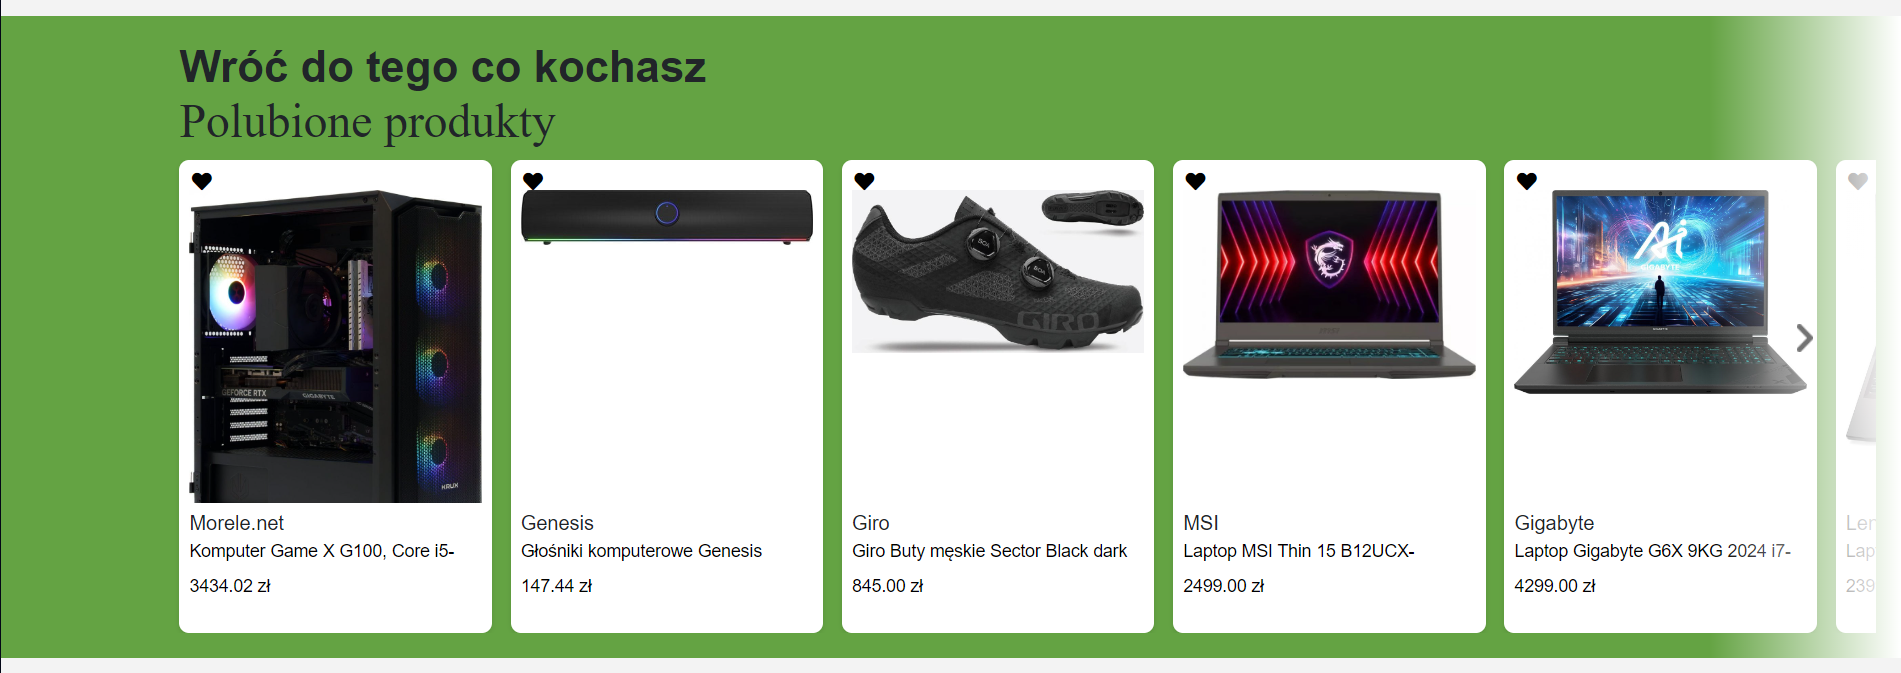
\includegraphics[width=0.7\columnwidth]{images/krzysztofBImages/slider-ulubione.png}
        \caption{Slider z polecanymi i polubionymi}
        \emph{Źródło: opracowanie własne.}
    \end{figure}

    \begin{figure}[H]
        \centering
        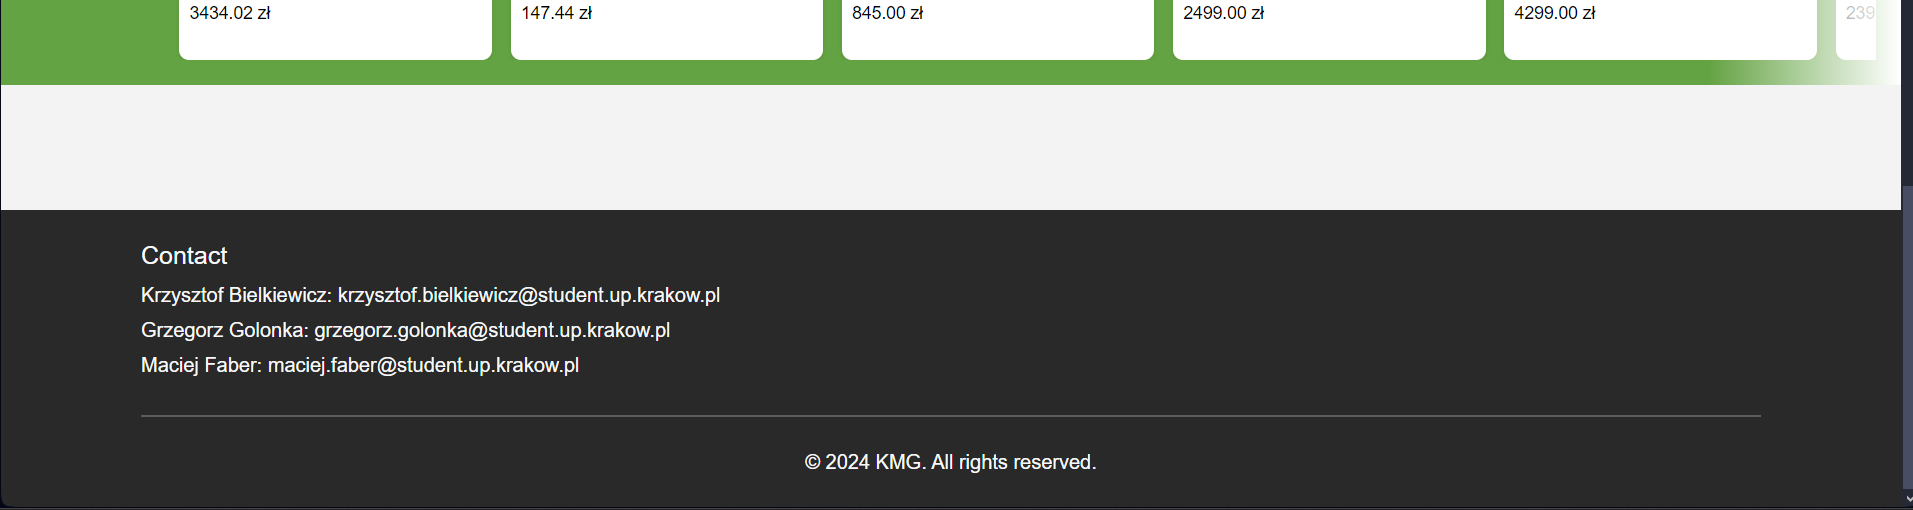
\includegraphics[width=0.7\columnwidth]{images/krzysztofBImages/footer.png}
        \caption{Stopka}
        \emph{Źródło: opracowanie własne.}
    \end{figure}


\subsubsection{Krzysztof Bielkiewicz: Opcja wyszukiwania po słowach kluczowych}
\label{1.3.3}
\textit{Implementacja w backend wyszukiwania po słowach wpisanych w rubryce 'Szukaj'
oraz strona wyświetlająca wynik wyszukiwania i jej oprawa graficzna.}
\begin{figure}[H]
    \centering
    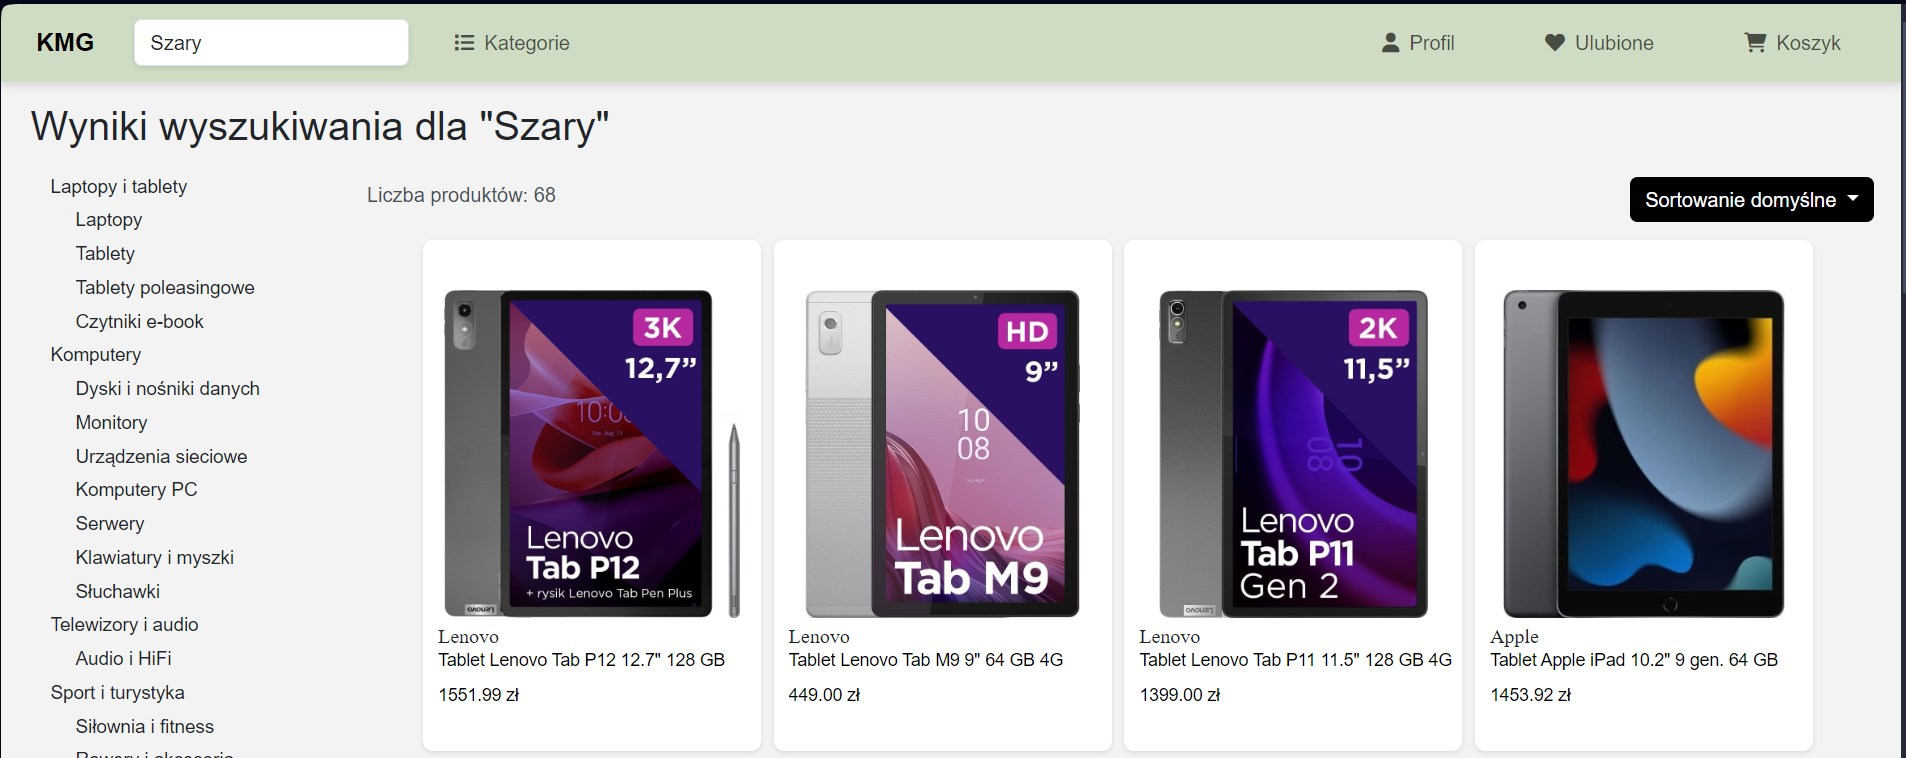
\includegraphics[width=0.8\columnwidth]{images/krzysztofBImages/wyszukiwanie.png}
    \caption{Wynik wyszukiwania}
    \emph{Źródło: opracowanie własne.}
\end{figure}

    
\subsubsection{Krzysztof Bielkiewicz: Opcja wyszukiwania po kategoriach}
\label{1.3.4}
    \textit{Zaimplementowana w backend opcja wyszukiwania po kategoriach
     oraz stworzenie w frontend liste kategorii w nagłówku
      oraz liste kategorii po lewej stronie od wyświetlanych produktów w której jest zaznaczona
      aktualnie przeglądana kategoria. Utworzenie strony z wyświetlanymi produktami z wybranej kategorii.}
    \begin{center}
        \hyperref[header-categories]{Zdjęcie wyszukiwania po kategoriach w nagłówku}
    \end{center}

    \begin{figure}[H]
        \centering
        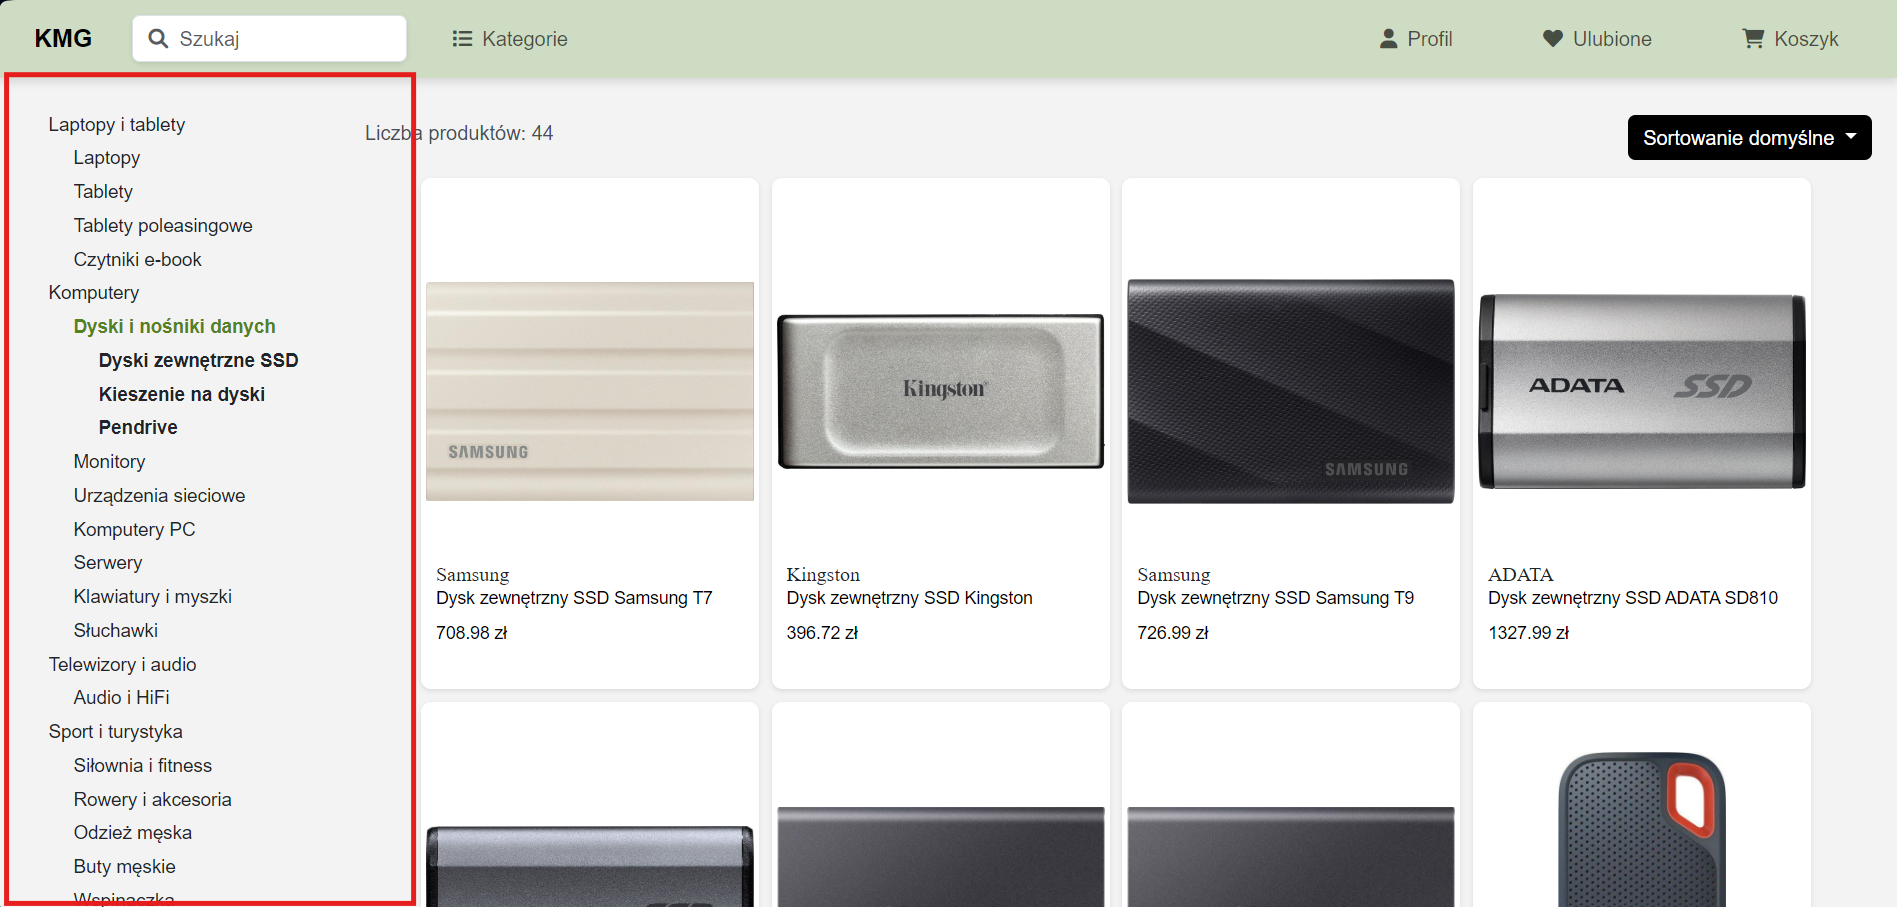
\includegraphics[width=0.8\columnwidth]{images/krzysztofBImages/lewe-kategorie.png}
        \caption{Kategorie po lewej stronie na stronie z produktami z wybranej kategorii}
        \emph{Źródło: opracowanie własne.}
    \end{figure}


\subsubsection{Krzysztof Bielkiewicz: Stworzenie strony z ulubionymi produktami}
\label{1.3.5}
\textit{Strona wyświetlająca produkty polubione przez użytkownika/lub w danej sesji.}

\begin{figure}[H]
    \centering
    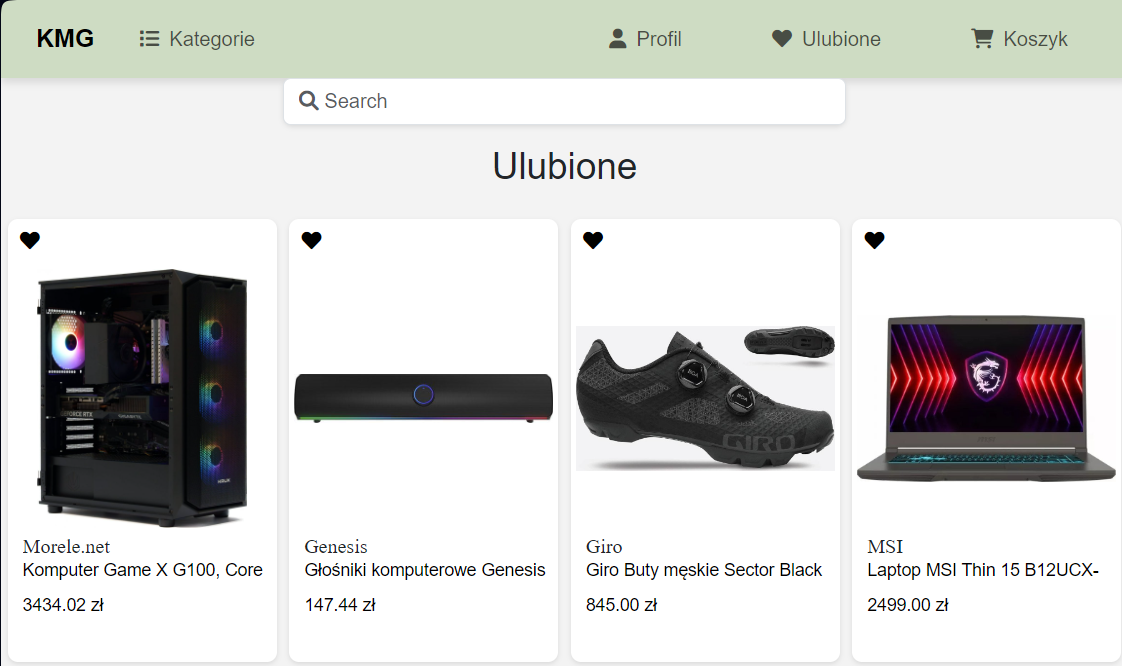
\includegraphics[width=0.8\columnwidth]{images/krzysztofBImages/strona-ulubione.png}
    \caption{Strona z polubionymi produktami}
    \emph{Źródło: opracowanie własne.}
\end{figure}

\subsubsection{Krzysztof Bielkiewicz: Stworzenie strony profilu z opcją edycji}
\label{1.3.6}
\textit{Stworzenie responsywnej strony w backend i frontend do edycji danych z modelu User.
Umożliwia edycje podstawych danych jak e-mail, imię, date urodzenia, itp.
Oraz umożliwia zmianę hasła.}

\begin{figure}[H]
    \centering
    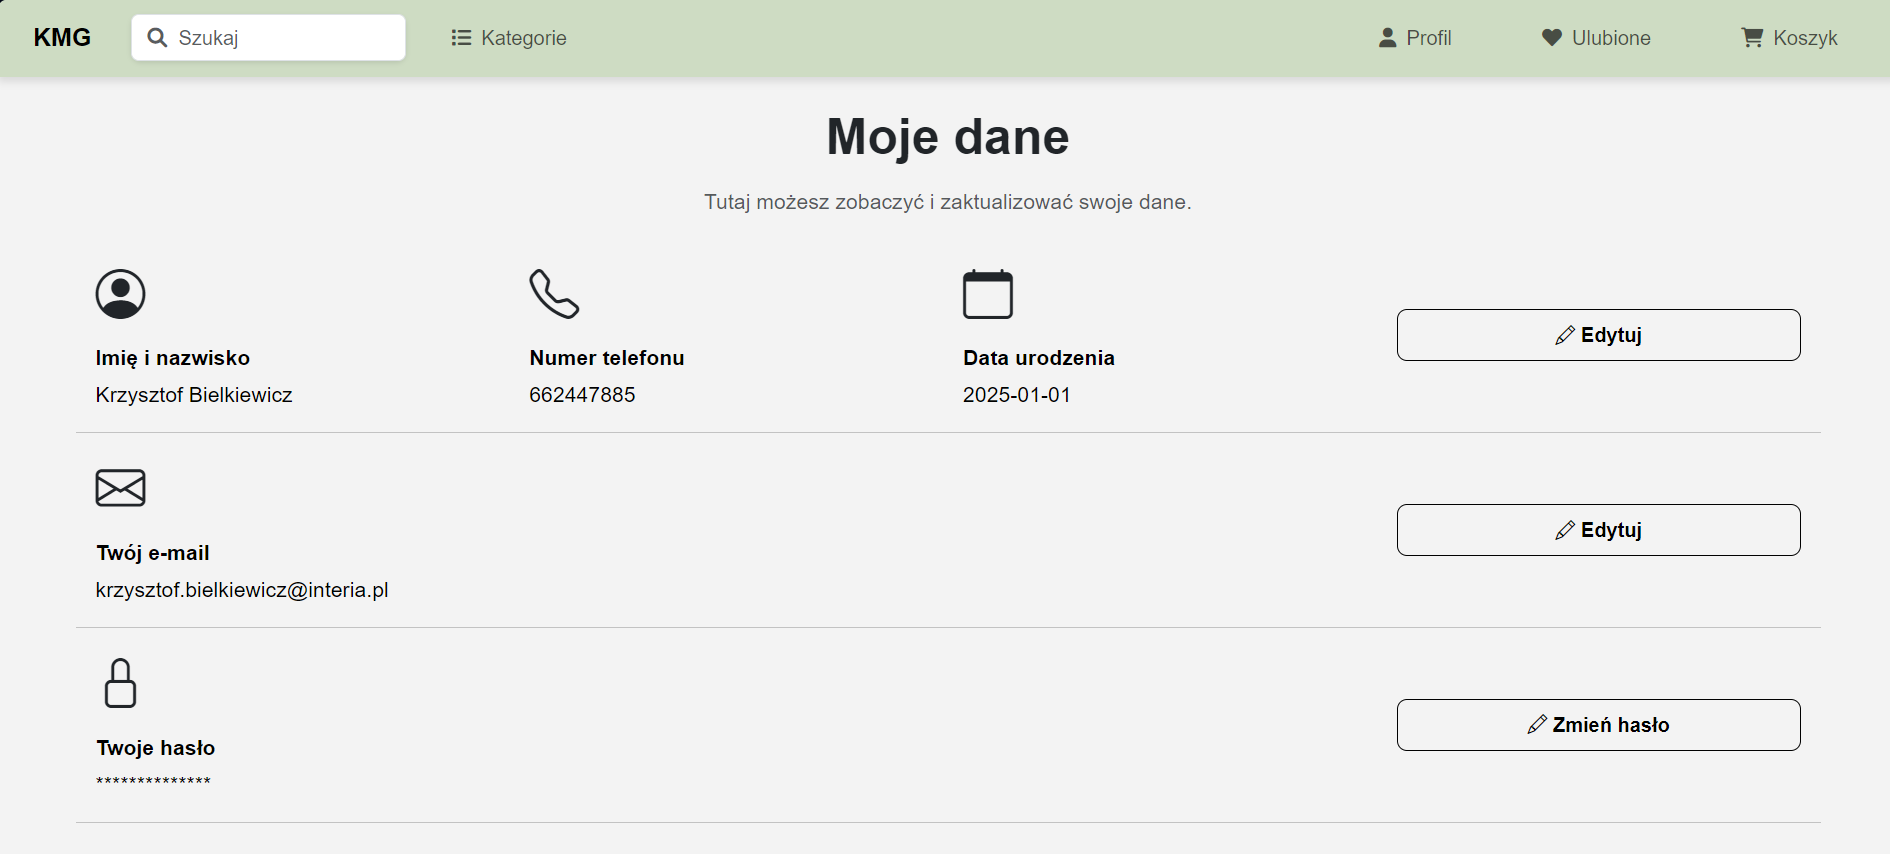
\includegraphics[width=0.9\columnwidth]{images/krzysztofBImages/profil/strona-edycji-profilu.png}
    \caption{Strona z polami do edycji profilu}
    \emph{Źródło: opracowanie własne.}
\end{figure}

\begin{figure}[H]
    \centering
    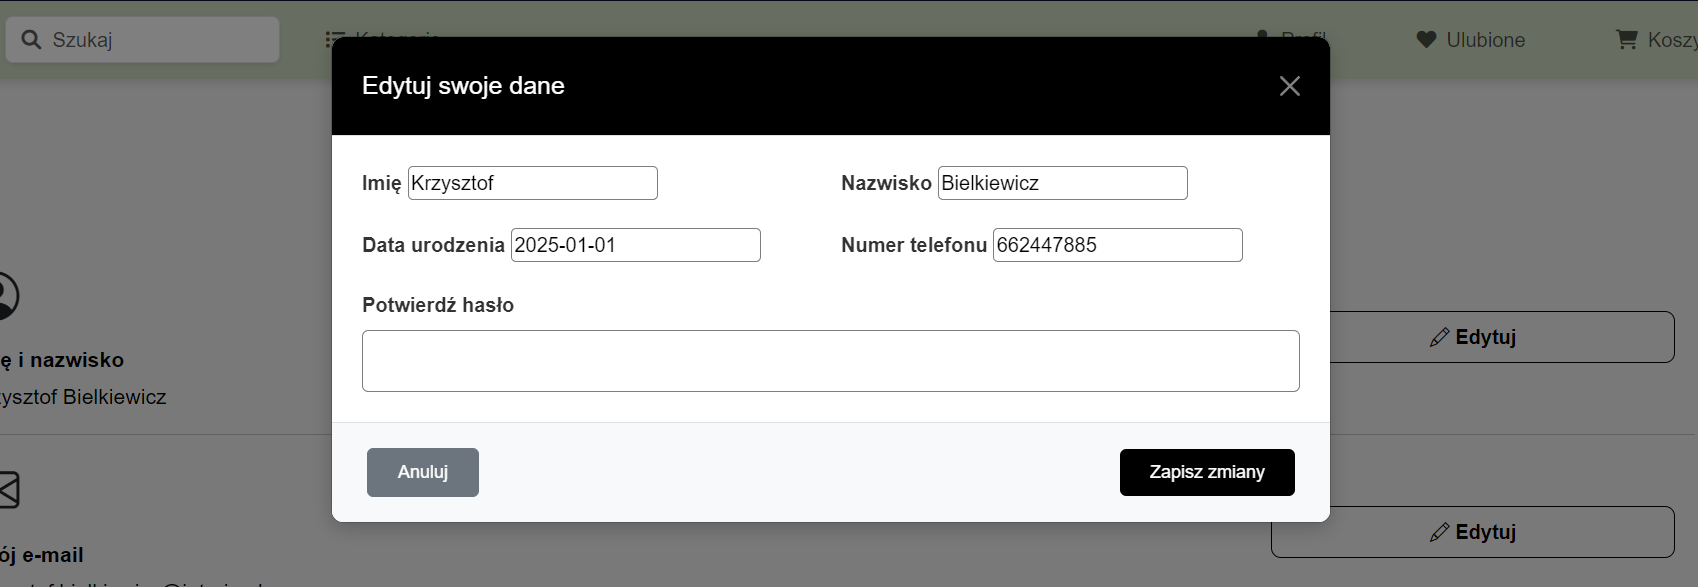
\includegraphics[width=0.9\columnwidth]{images/krzysztofBImages/profil/edycja-danych.png}
    \caption{Formularz edytowania podstawowych danych}
    \emph{Źródło: opracowanie własne.}
\end{figure}

\begin{figure}[H]
    \centering
    \includegraphics[width=0.9\columnwidth]{images/krzysztofBImages/profil/zmiana-hasła.png}
    \caption{Formularz zmiany hasła}
    \emph{Źródło: opracowanie własne.}
\end{figure}

\begin{figure}[H]
    \centering
    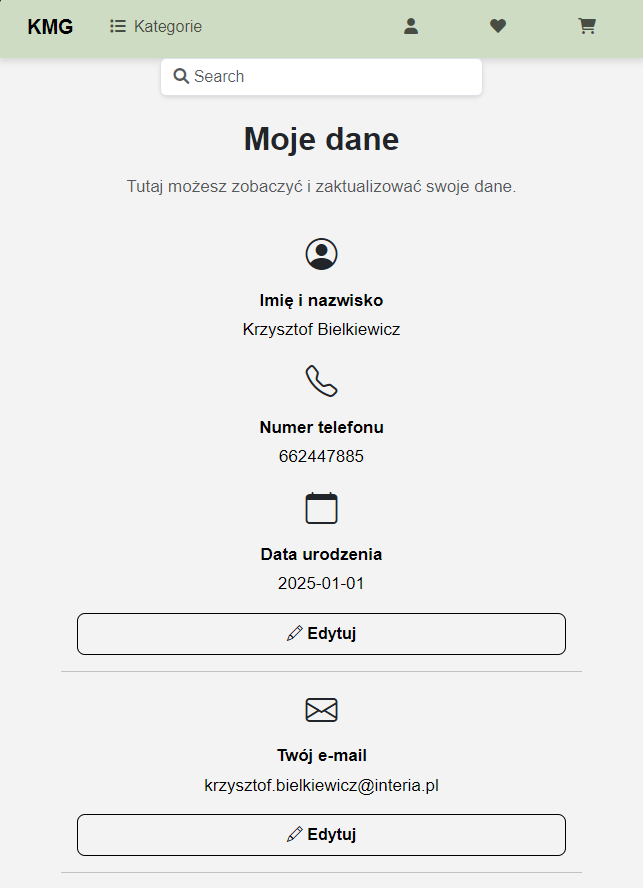
\includegraphics[width=0.5\columnwidth]{images/krzysztofBImages/profil/responywna-strona-profilu.png}
    \caption{Responywna strona edycji profilu}
    \emph{Źródło: opracowanie własne.}
\end{figure}

\subsubsection{Krzysztof Bielkiewicz: Oprawa graficzna strony adresu dostawy}
\label{1.3.7}
\textit{Utworzenie oprawy graficznej dla strony dodania adresu dostawy.}
\begin{figure}[H]
    \centering
    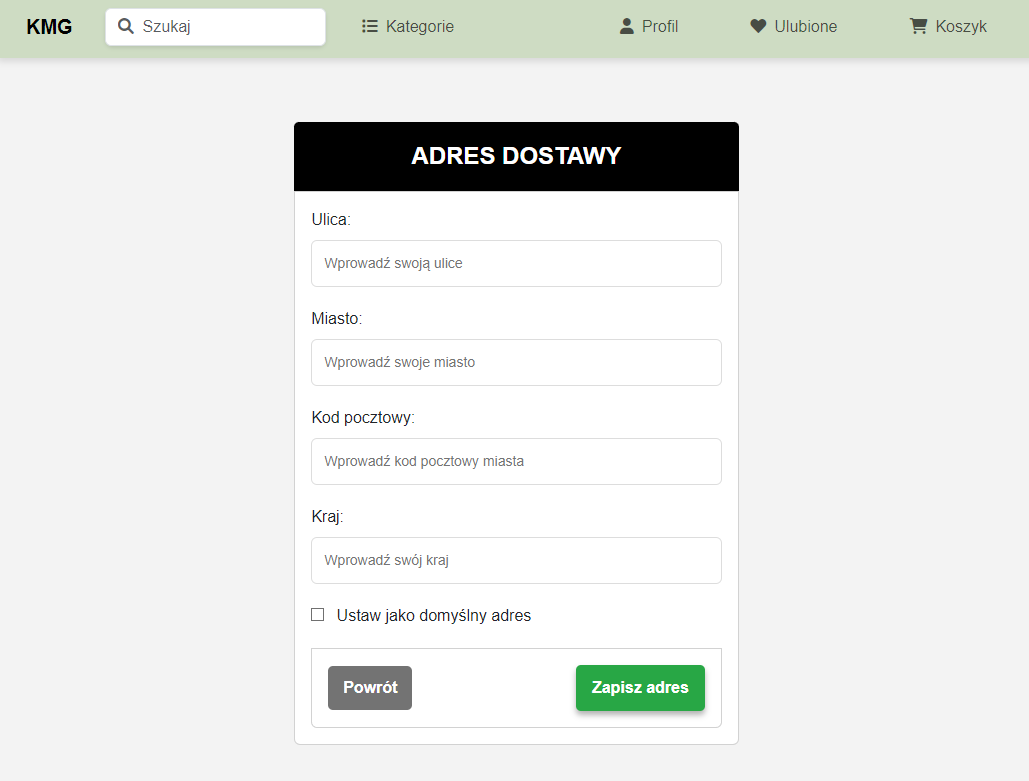
\includegraphics[width=0.8\columnwidth]{images/krzysztofBImages/strona-dodaj-adres.png}
    \caption{Strona z formularzem dodania adresu dostawy}
    \emph{Źródło: opracowanie własne.}
\end{figure}

\subsubsection{Krzysztof Bielkiewicz: Oprawa graficzna koszyka}
\label{1.3.8}
\textit{Utworzenie oprawy graficznej dla koszyka i jej responywność.}
\begin{figure}[H]
    \centering
    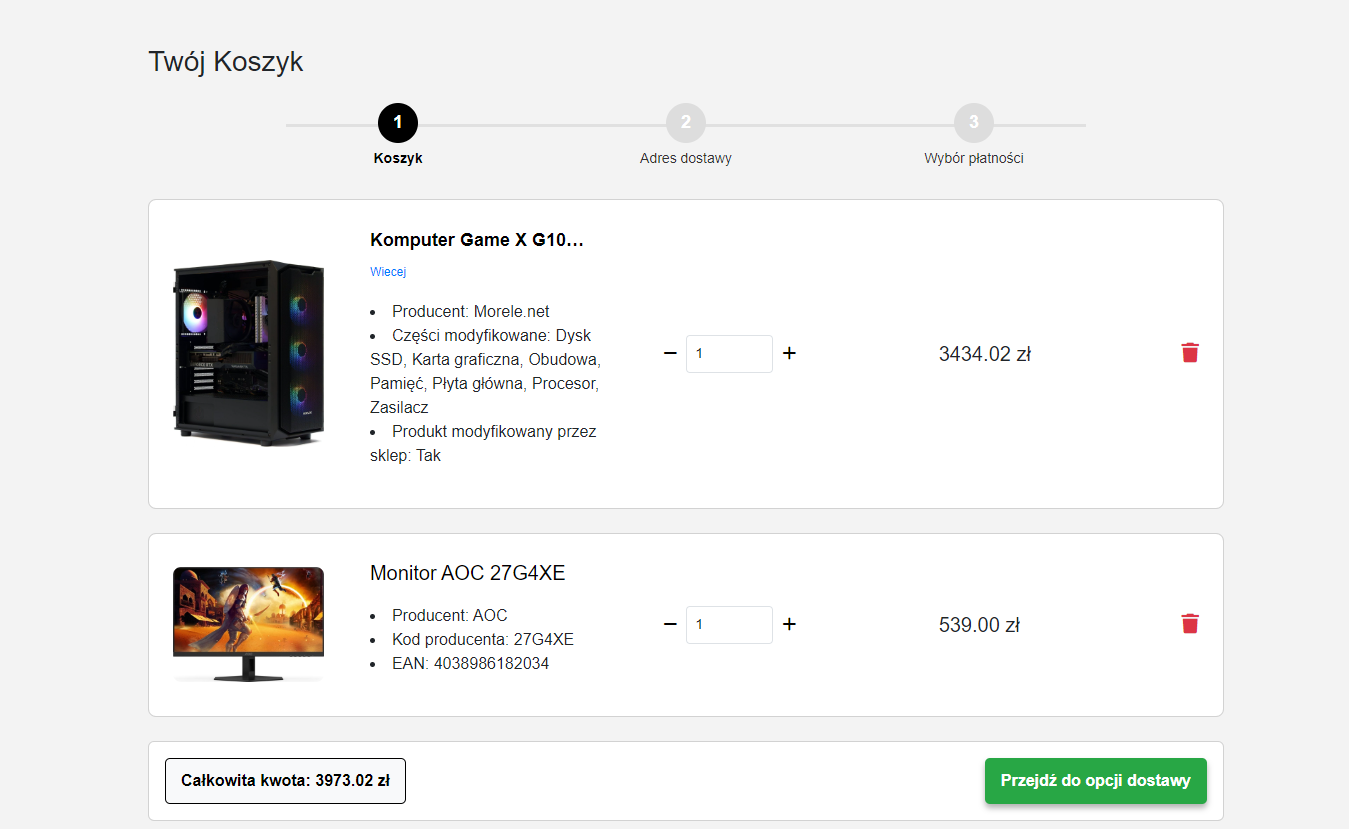
\includegraphics[width=0.8\columnwidth]{images/krzysztofBImages/cart/cart-step1.png}
    \caption{Strona koszyka}
    \emph{Źródło: opracowanie własne.}
\end{figure}

\begin{figure}[H]
    \centering
    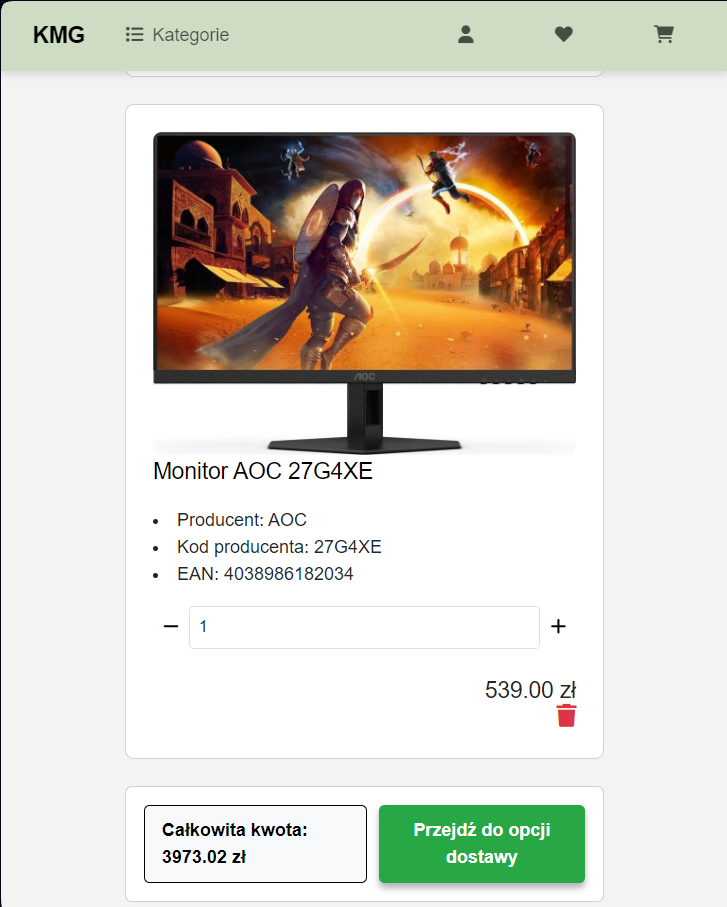
\includegraphics[width=0.5\columnwidth]{images/krzysztofBImages/cart/cart-step1-respo.png}
    \caption{Strona koszyka - responsywna}
    \emph{Źródło: opracowanie własne.}
\end{figure}

\subsubsection{Krzysztof Bielkiewicz: Oprawa graficzna wyboru adresu dostawy}
\label{1.3.9}
\textit{Utworzenie oprawy graficznej dla wyboru adresu dostawy.}
\begin{figure}[H]
    \centering
    \includegraphics[width=0.8\columnwidth]{images/krzysztofBImages/cart/wybór-adresu-dostawy.png}
    \caption{Strona wyboru adresu dostawy}
    \emph{Źródło: opracowanie własne.}
\end{figure}

\subsubsection{Krzysztof Bielkiewicz: Oprawa graficzna dla metod płatności}
\label{1.3.10}
\textit{Utworzenie oprawy graficznej metod płatności.}
\begin{figure}[H]
    \centering
    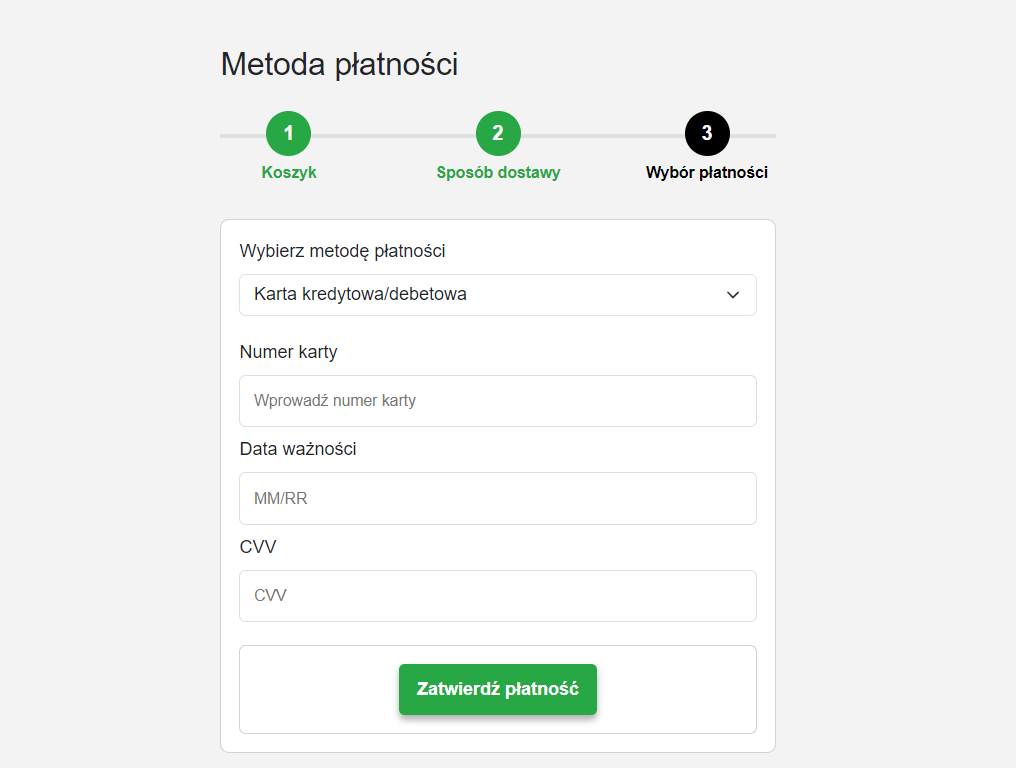
\includegraphics[width=0.8\columnwidth]{images/krzysztofBImages/cart/metody-płatności-karta.png}
    \caption{Metoda płatności kartą}
    \emph{Źródło: opracowanie własne.}
\end{figure}

\begin{figure}[H]
    \centering
    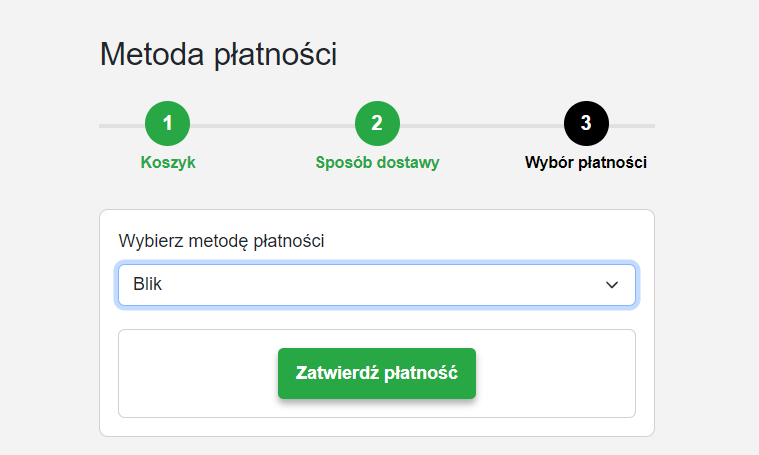
\includegraphics[width=1.0\columnwidth]{images/krzysztofBImages/cart/metody-płatności-blik.png}
    \caption{Metoda płatności blik}
    \emph{Źródło: opracowanie własne.}
\end{figure}

\begin{figure}[H]
    \centering
    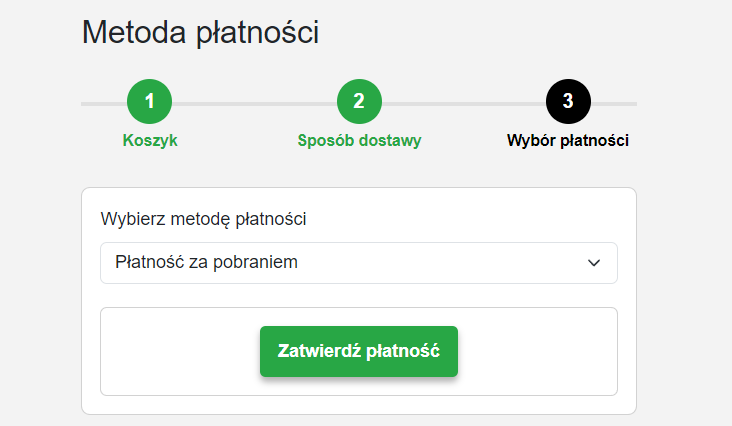
\includegraphics[width=0.8\columnwidth]{images/krzysztofBImages/cart/metody-płatności-za-pobraniem.png}
    \caption{Metoda płatności za pobraniem}
    \emph{Źródło: opracowanie własne.}
\end{figure}

\subsubsection{Krzysztof Bielkiewicz: Oprawa graficzna szczegółów zamówienia}
\label{1.3.11}
\textit{Utworzenie oprawy graficznej dla strony ze szegółami zamówienia i jej responywność.}

\begin{figure}[H]
    \centering
    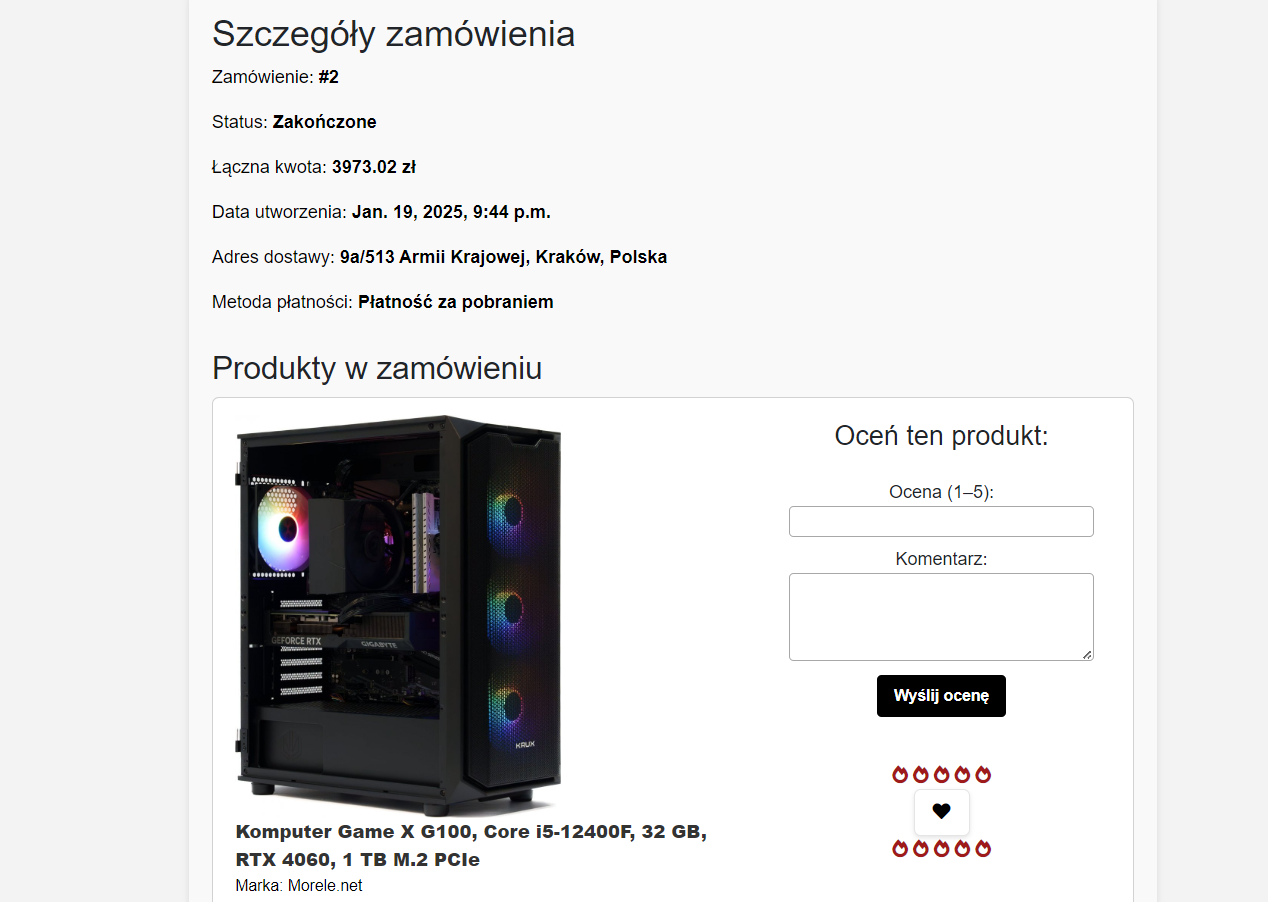
\includegraphics[width=0.8\columnwidth]{images/krzysztofBImages/szczegóły-zamówieniaV1.png}
    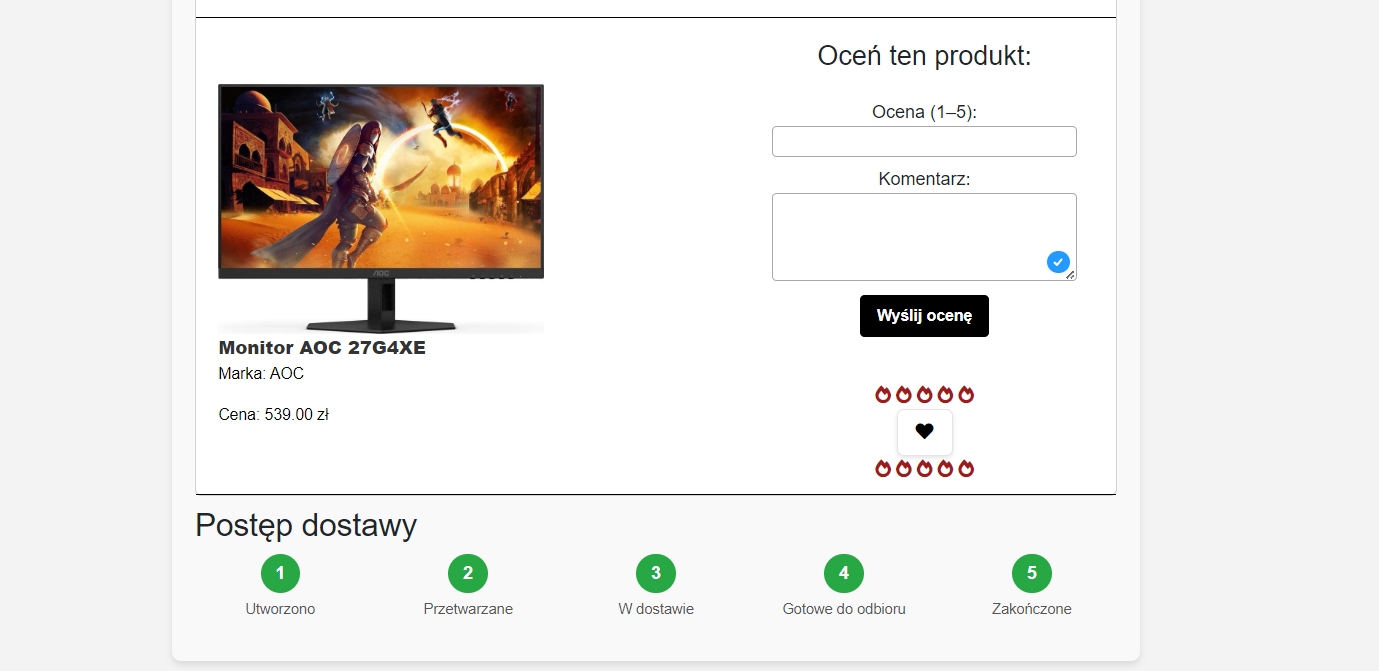
\includegraphics[width=0.8\columnwidth]{images/krzysztofBImages/szczegóły-zamówieniaV2.png}
    \caption{Strona ze szegółami zamówienia}
    \emph{Źródło: opracowanie własne.}
\end{figure}

\begin{figure}[H]
    \centering
    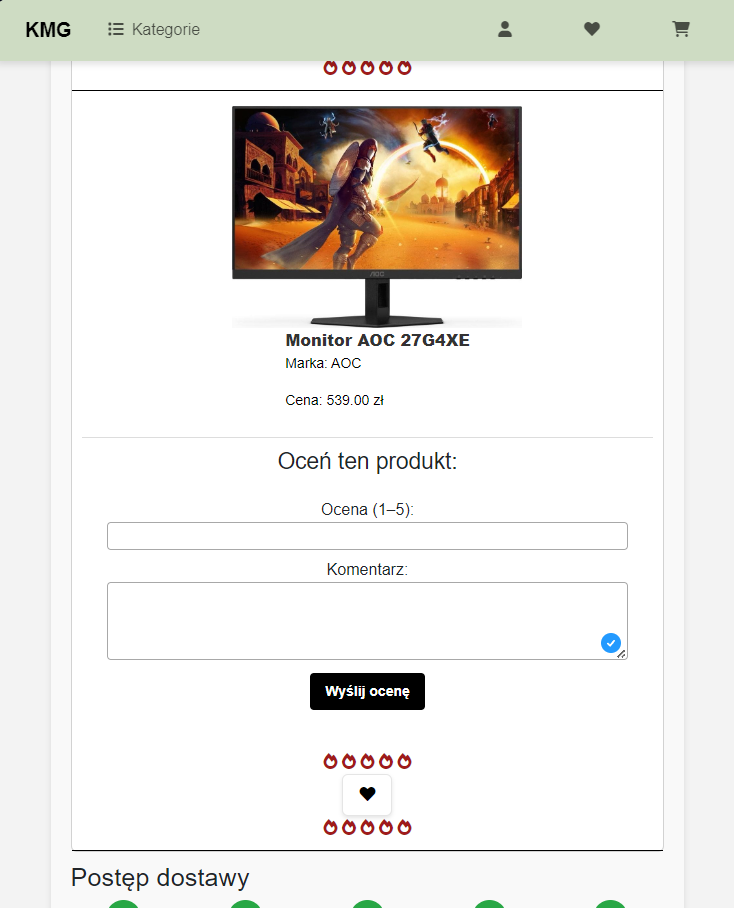
\includegraphics[width=0.5\columnwidth]{images/krzysztofBImages/szczegóły-zamówienia-respo.png}
    \caption{Responywna strona ze szegółami zamówienia}
    \emph{Źródło: opracowanie własne.}
\end{figure}

\subsubsection{Krzysztof Bielkiewicz: Oprawa graficzna dla listy zamówień}
\label{1.3.12}
\textit{Utworzenie oprawy graficznej dla listy zamówień.}

\begin{figure}[H]
    \centering
    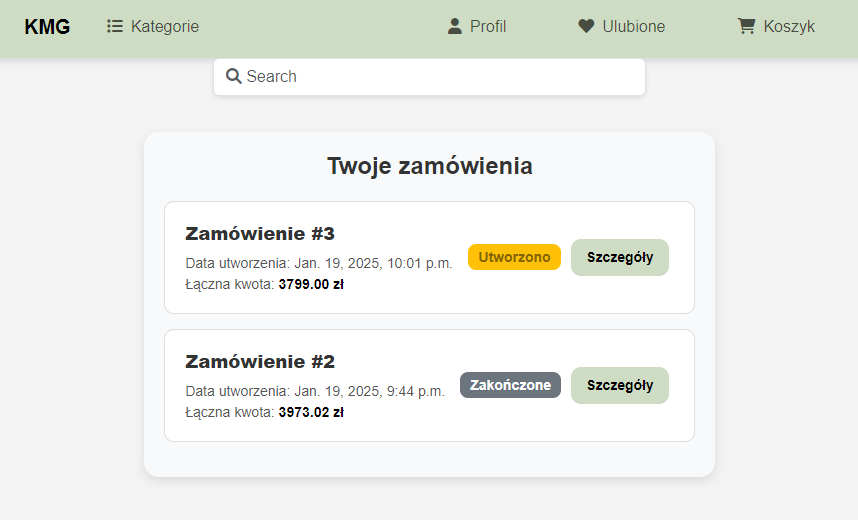
\includegraphics[width=0.8\columnwidth]{images/krzysztofBImages/orders.png}
    \caption{Lista zamówień}
    \emph{Źródło: opracowanie własne.}
\end{figure}


\subsubsection{Krzysztof Bielkiewicz: Wyświetlenie produktów z bazy danych}
\label{1.3.13}
\textit{Utworzenie strony wyświetlającej produkty z podstawowymi danymi: marka, tytuł, cena oraz zdjęcie.
Przyciski polubienia i koszyka dla każdego produktu po najechaniu na dany produkt.
Produkty polubione przez użytkownika mają widoczne serca.
Oprawa graficzna dla wyświetlanych prduktów i przycisków polubienia i dodania do koszyka.}
\begin{figure}[H]
    \centering
    \includegraphics[width=0.9\columnwidth]{images/krzysztofBImages/lista-produktów.png}
    \caption{Wyświetlanie listy produktów}
    \emph{Źródło: opracowanie własne.}
\end{figure}

\begin{figure}[H]
    \centering
    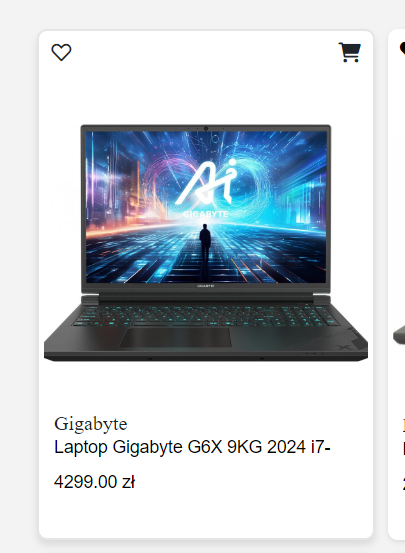
\includegraphics[width=0.5\columnwidth]{images/krzysztofBImages/przyciski-polubienia-koszyka.png}
    \caption{Przyciski polubienia i dodania do koszyka.}
    \emph{Źródło: opracowanie własne.}
\end{figure}

\begin{figure}[H]
    \centering
    \includegraphics[width=0.5\columnwidth]{images/krzysztofBImages/lista-produktów-respo.png}
    \caption{Wyświetlanie listy produktów - responywność}
    \emph{Źródło: opracowanie własne.}
\end{figure}



\subsubsection{Krzysztof Bielkiewicz: Funkcja dodawania produktów do ulubionych}
\label{1.3.14}
\textit{Dodawanie produktów do ulubionych i usuwanie ich z ulubionych przy użyciu django.
Produkt po kliknięciu na przycisk sreca dodaje się do Ulubionych i za poconą skrytu 
JavaScript zmienia ikonke serca na czarne wypełnione. Dane produkty pojawiają się na stronie Ulubione.
Po kliknięciu z powrotem na wypełnione serce produkt usuwa się ulubionych.
Produkty polubione zapisują się w danej sesji i po zalogowaniu są wysyłane do polubień danego usera,
co zapewnia wygode dla użytkownika.}


\subsubsection{Krzysztof Bielkiewicz: Paginacja produktów na stronach}
\label{1.3.15}
\textit{Paginacja dla stron 'Wszystkie produkty', 'Produkty z kategorii', 'Wyszukane produkty', 'Ulubione'.}
\begin{figure}[H]
    \centering
    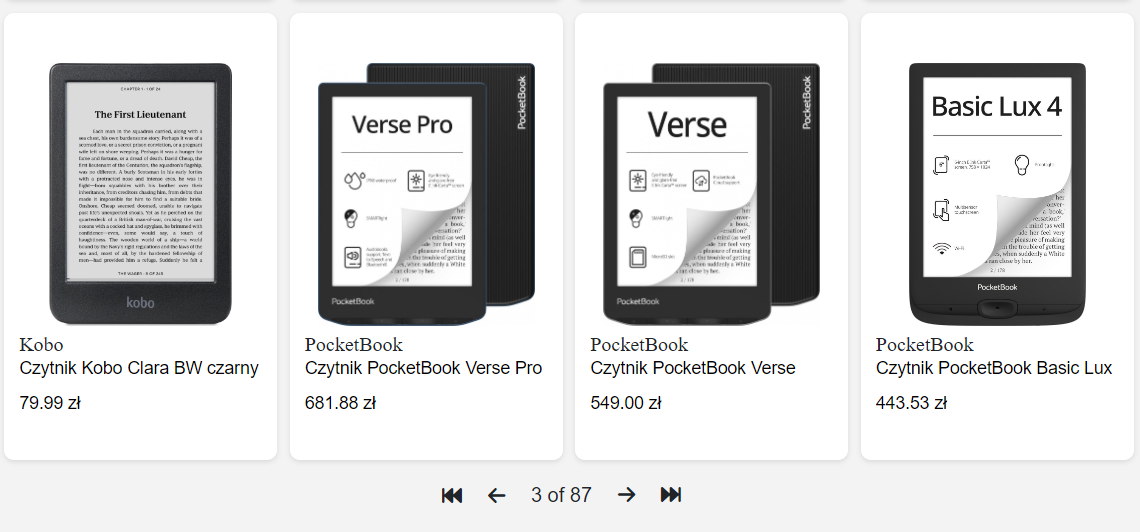
\includegraphics[width=1.0\columnwidth]{images/krzysztofBImages/pagination.png}
    \caption{Paginacja}
    \emph{Źródło: opracowanie własne.}
\end{figure}


\subsubsection{Krzysztof Bielkiewicz: Oprawa graficzna szczegółów produktu}
\label{1.3.16}
\textit{Oprawa graficzna dla szegółów produktu i jej responywność.}
\begin{figure}[H]
    \centering
    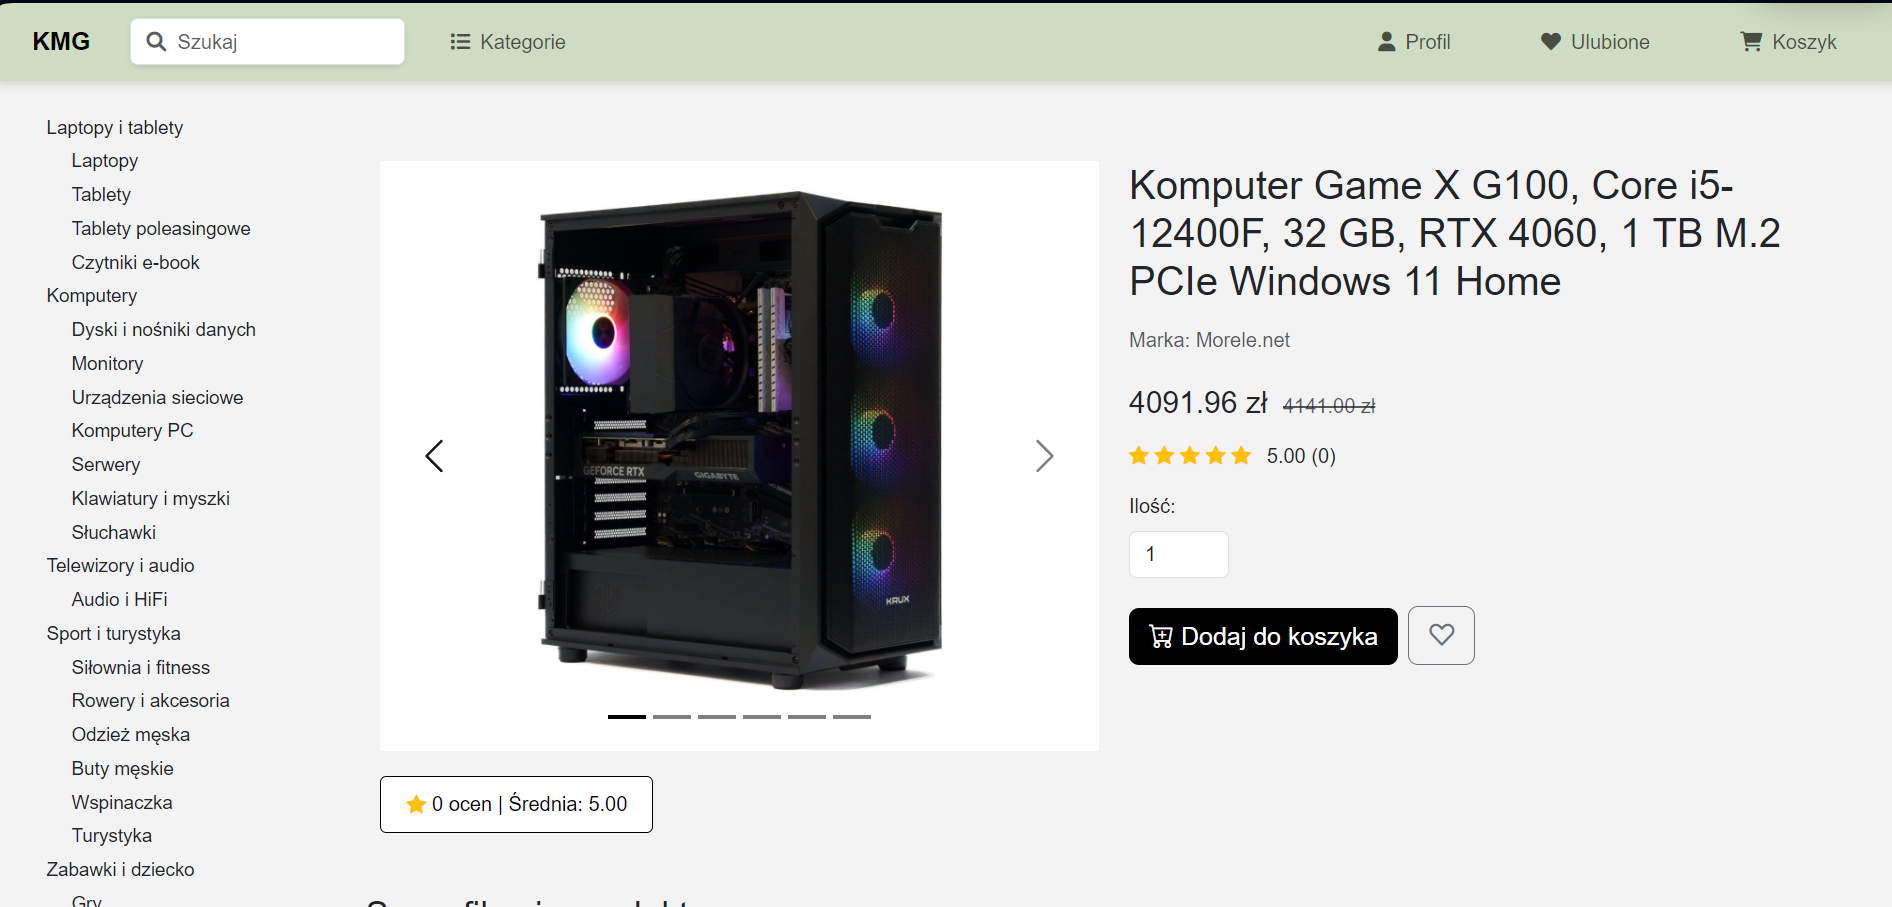
\includegraphics[width=1.0\columnwidth]{images/krzysztofBImages/product-detail.png}
    \caption{Szczegóły produkt}
    \emph{Źródło: opracowanie własne.}
\end{figure}
\begin{figure}[H]
    \centering
    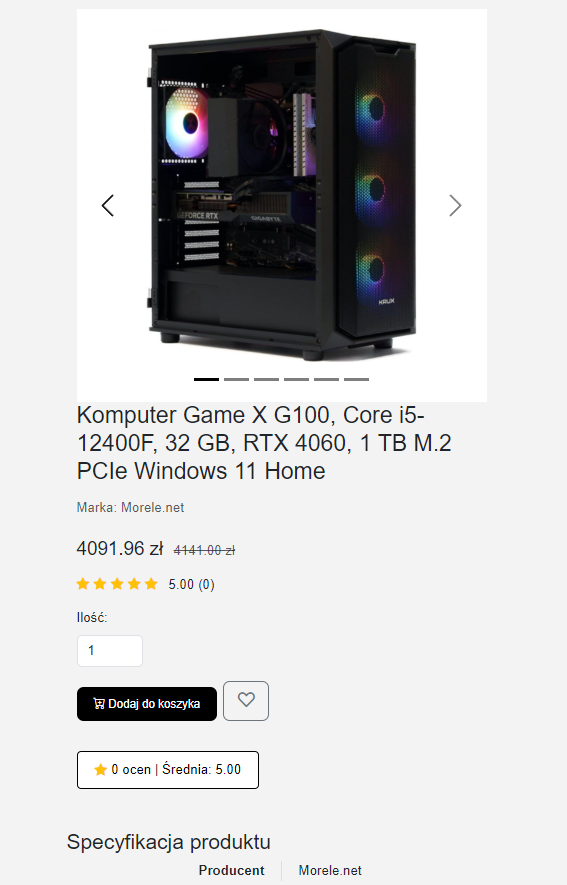
\includegraphics[width=0.5\columnwidth]{images/krzysztofBImages/product-detail-respo.png}
    \caption{Szczegóły produkt - responywna wersja}
    \emph{Źródło: opracowanie własne.}
\end{figure}

\subsubsection{Krzysztof Bielkiewicz: Custom errory i oprawa graficzna rejestracji}
\label{1.3.17}
\textit{Własne errory wyświetlające się pod wymaganymi polami,
pole telefonu z automatycznym formatem zrobionym w JS,
 wybór daty urodzenia z zablokowanym wyborem daty w przyszłości (JS). Oprawa graficzna.
 Oraz okienko powiadamiające o udanej rejestracji.}

\begin{figure}[H]
    \centering
    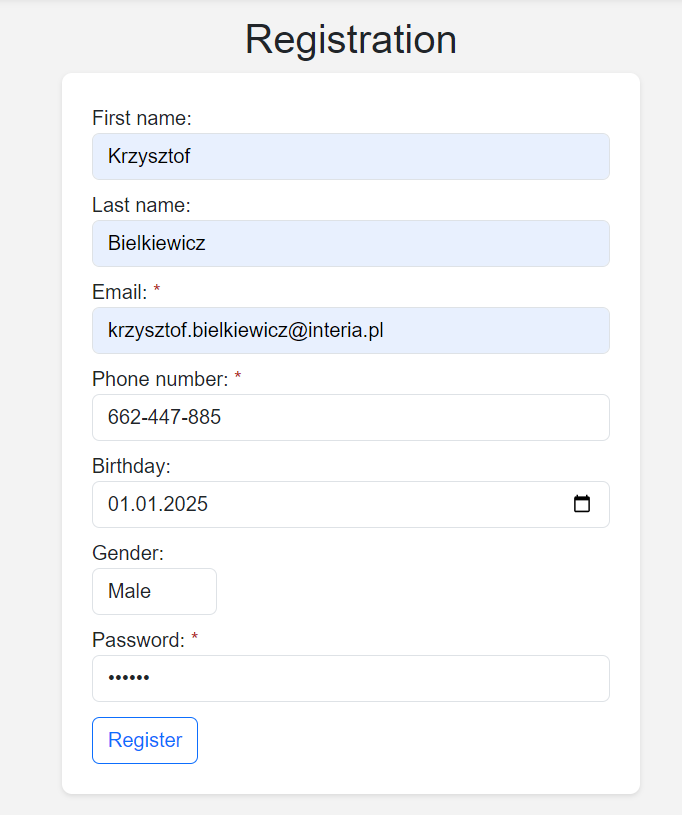
\includegraphics[width=0.5\columnwidth]{images/krzysztofBImages/register-login/registration.png}
    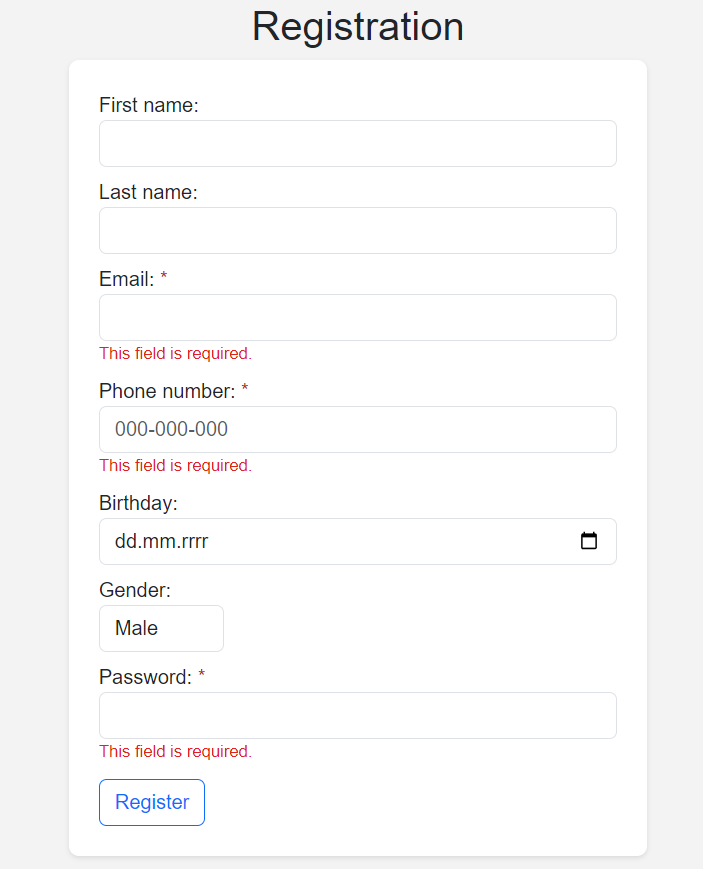
\includegraphics[width=0.48\columnwidth]{images/krzysztofBImages/register-login/register-errors.png}
    \caption{Rejestracja}
    \emph{Źródło: opracowanie własne.}
\end{figure}
\begin{figure}[H]
    \centering
    
\includegraphics[width=0.6\columnwidth]{images/krzysztofBImages/register-login/message.png}
    \caption{Powiadomienie}
    \emph{Źródło: opracowanie własne.}
\end{figure}


\subsubsection{Krzysztof Bielkiewicz: Custom errory i oprawa graficzna loginu}
\label{1.3.18}
\textit{Oprawa graficzna. Własne errory wyświetlające się pod wymaganymi polami.}

\begin{figure}[H]
    \centering
    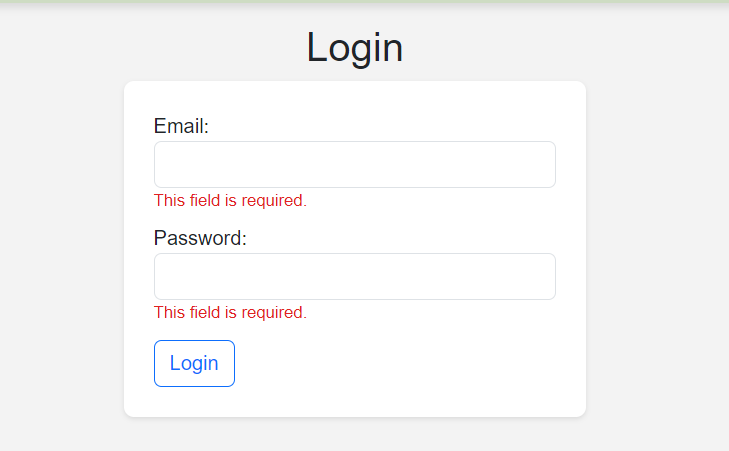
\includegraphics[width=0.8\columnwidth]{images/krzysztofBImages/register-login/login.png}
    \caption{Login}
    \emph{Źródło: opracowanie własne.}
\end{figure}



%  Zadania Grzegorz Golonka
\subsubsection{Grzegorz Golonka: Utworzenie pliku README.md }
\label{section:1.3.19}
\textit{Przygotowanie szczegółowego pliku README.md dla projektu \texttt{kmg\_store},
 zawierającego opis projektu, spis treści, funkcjonalności,
 modele bazodanowe oraz instrukcję instalacji i użycia aplikacji.
Plik README.md został stworzony w sposób przejrzysty i intuicyjny,
co ułatwia zrozumienie struktury projektu oraz jego uruchomienie przez nowych użytkowników i deweloperów.}
\begin{figure}[H]
    \centering
    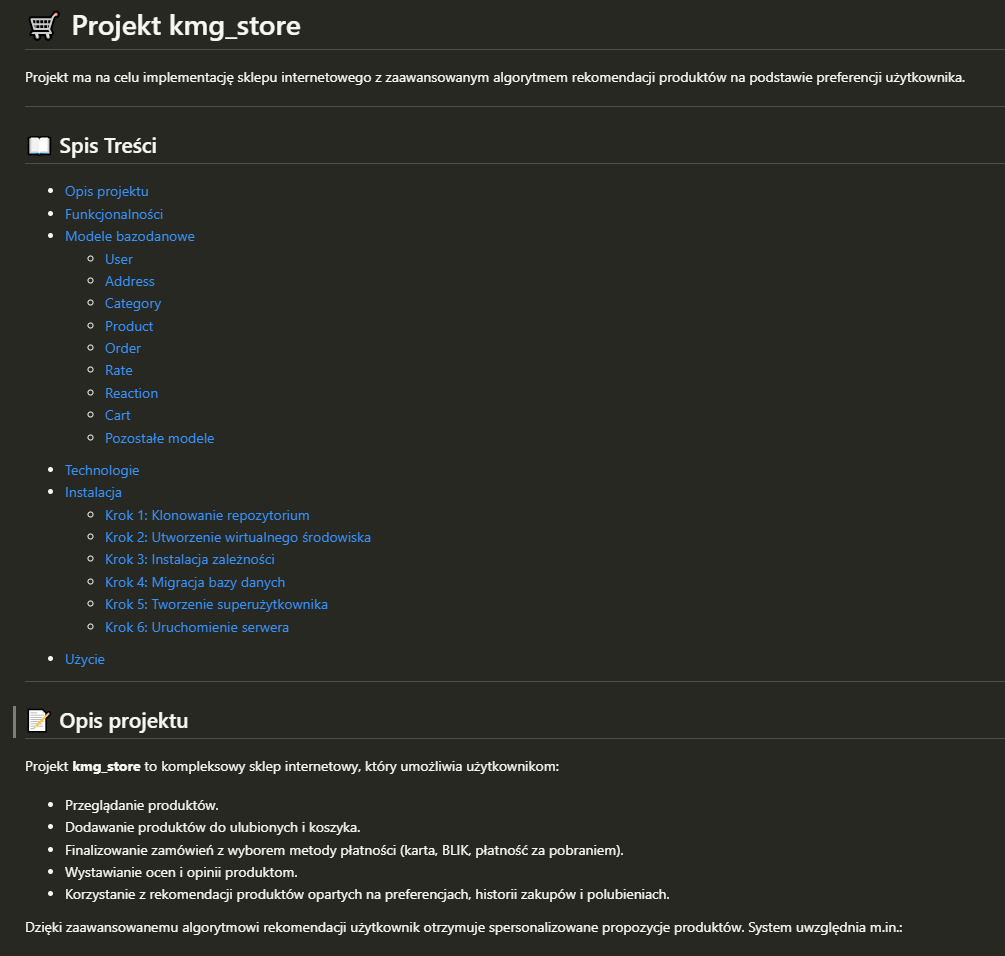
\includegraphics[width=0.9\columnwidth]{images/krzysztofBImages/readme_preview.png}
    \caption{Widok pliku README.md dla projektu \textbf{kmg\_store}}
    \emph{Źródło: opracowanie własne.}
\end{figure}
%
%
\subsubsection{Grzegorz Golonka: Utworzenie modeli bazodanowych}
\label{section:1.3.20}
Przygotowanie głównych modeli bazodanowych dla projektu \texttt{kmg\_store}.
W ramach tego zadania zaimplementowano struktury danych w pliku \texttt{models.py},
obejmujące m.in. modele użytkowników (\texttt{User}), adresów dostawy (\texttt{Address}),
metod płatności (\texttt{PaymentMethod}), kategorii produktów (\texttt{Category}),
zamówień (\texttt{Order}), produktów (\texttt{Product}) oraz dodatkowe modele wspierające
takie jak reakcje użytkowników (\texttt{Reaction}) czy modele (\texttt{Conversation}).

Modele zostały zaprojektowane zgodnie z wymaganiami projektu, uwzględniając relacje między tabelami,
walidację danych oraz dodatkowe funkcje wspierające, takie jak obliczanie średniej oceny produktu,
zarządzanie ulubionymi produktami czy obsługa historii interakcji użytkownika.
Dzięki temu stworzono elastyczną i wydajną strukturę bazy danych,
umożliwiającą rozwój funkcjonalności sklepu internetowego w przyszłości.

\begin{figure}[H]
    \centering
    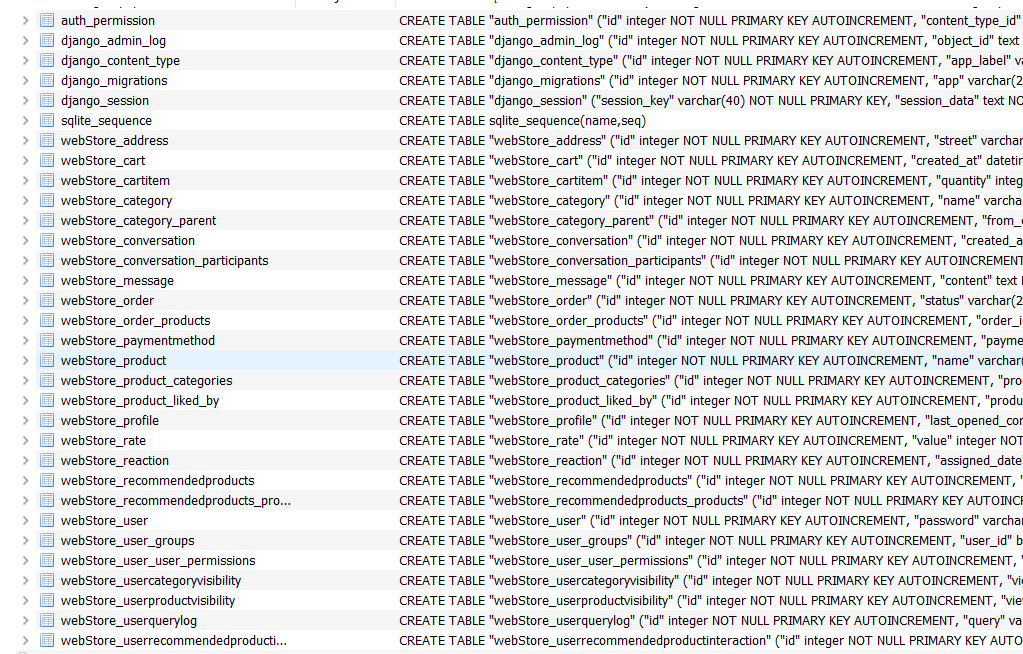
\includegraphics[width=0.9\columnwidth]{images/krzysztofBImages/modele_bazodanowe.png}
    \caption{Widok tabel w przeglądarce DB Browser for SQLite}
    \emph{Źródło: opracowanie własne.}
    \label{fig:db_models}
\end{figure}


%
%
\subsubsection{Grzegorz Golonka: Dodanie skryptów do inicjalizacji projektu}
\label{section:1.3.21}
Dodanie skryptów wspierających inicjalizację projektu \texttt{kmg\_store}. W ramach tego zadania przygotowano dwa główne skrypty:

\begin{itemize}
    \item \texttt{create\_superuser.py} – Skrypt umożliwiający automatyczne tworzenie konta superużytkownika. Skrypt weryfikuje, czy konto z określonym loginem już istnieje, a jeśli nie, tworzy je z domyślnymi danymi.
    \item \texttt{init\_project\_bash.sh} – Skrypt powłokowy automatyzujący proces inicjalizacji środowiska projektu. Obejmuje m.in. tworzenie i aktywację wirtualnego środowiska, instalację zależności, zarządzanie migracjami oraz uruchamianie serwera Django.
    \item \texttt{init\_project\_shell.ps} – Adekwatny skrypt do \texttt{init\_project\_bash.sh}, ale w wersji shellowej.
\end{itemize}

Skrypty te znacząco upraszczają proces przygotowania środowiska programistycznego, co przyczynia się do większej efektywności pracy zespołu.


Skrypty te znacząco upraszczają proces przygotowania środowiska programistycznego, co przyczynia się do większej efektywności pracy zespołu.
%
%
\subsubsection{Grzegorz Golonka: Stworzenie seeda produktów i kategorii}
\label{section:1.3.22}
\textit{
Przygotowanie skryptów do generowania danych testowych produktów i kategorii. Skrypty automatycznie pobierają dane z analizy znaczników HTML stron internetowych i zapisują je w formacie JSON. Zrealizowane zadania obejmują:
}
\begin{itemize}
    \item Pobieranie linków do produktów i tworzenie struktur kategorii.
    \item Zapisywanie szczegółowych danych produktów, takich jak nazwa, cena, zdjęcia i specyfikacje.
    \item Grupowanie i filtrowanie linków według wzorców.
\end{itemize}

\textit{
Skrypty te znacząco ułatwiają przygotowanie danych do testowania i wdrażania aplikacji.
}

\begin{figure}[H]
    \centering
    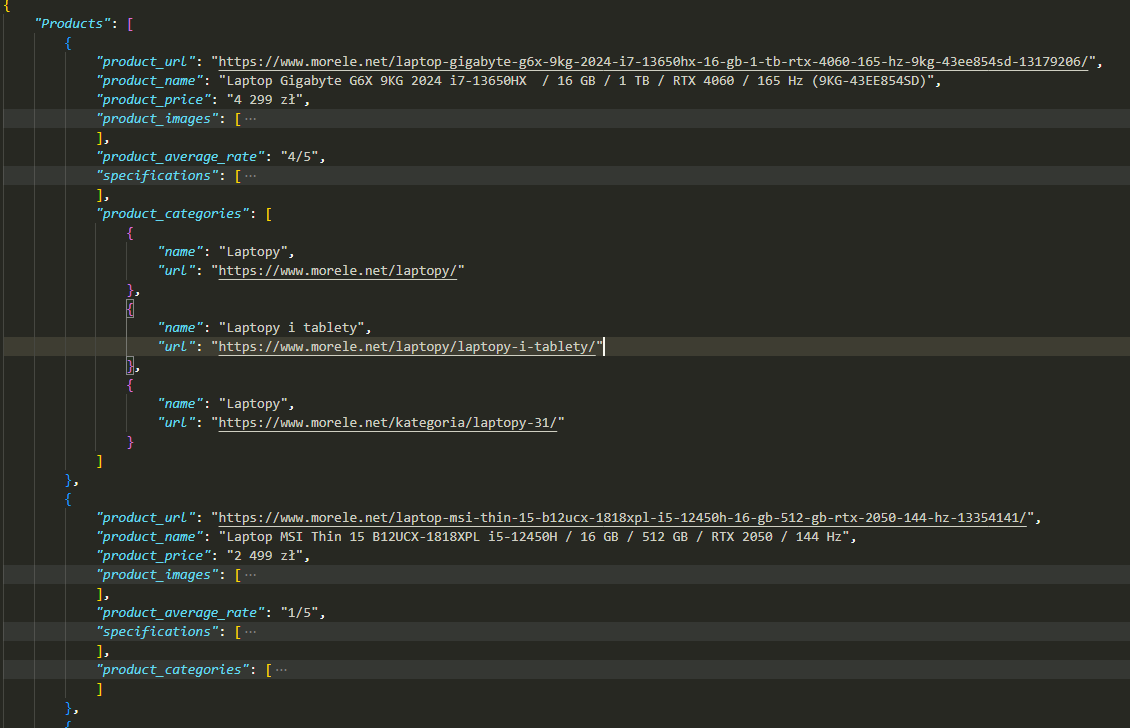
\includegraphics[width=0.9\columnwidth]{images/krzysztofBImages/products_seed.png}
    \caption{Przykładowy plik JSON z wygenerowanymi danymi produktów i kategorii}
    \emph{Źródło: opracowanie własne.}
\end{figure}
%
%
\subsubsection{Grzegorz Golonka: Formularze do modelów bazodanowych}
\label{section:1.3.23}
\textit{
Implementacja formularzy użytkownika w projekcie \texttt{kmg\_store} oraz ich integracja z widokami w celu obsługi rejestracji, logowania, adresów oraz metod płatności.
}

W ramach zadania stworzono i zaimplementowano następujące formularze:
\begin{itemize}
    \item \textbf{UserLoginForm} – formularz logowania użytkownika, obsługujący pola \texttt{email} i \texttt{password}. Formularz został zintegrowany z widokiem \texttt{UserLoginView}, umożliwiając autoryzację użytkownika oraz synchronizację danych sesji.
    \item \textbf{UserAddressForm} – formularz do zarządzania adresami użytkownika, umożliwiający zapis
     i odczyt danych adresowych (\texttt{street}, \texttt{city}, \texttt{postal\_code}, 
     \texttt{country}, \texttt{is\_default}). Formularz został użyty w widokach\\ \texttt{UserAddressCreationView} i \texttt{AddressSelectionView}, wspierając zarządzanie adresami oraz wybór domyślnego adresu dostawy.
    \item \textbf{PaymentMethodForm} – formularz obsługujący dodawanie metod płatności (karty kredytowe, Blik). Zawiera walidację 
    wymaganych pól w zależności od wybranej metody płatności. 
    Formularz zintegrowano z widokiem\\ \texttt{PaymentMethodView}, umożliwiając zapis metod płatności i obsługę kodów Blik.
    \item \textbf{UserRegistrationForm (częściowo)} – formularz rejestracyjny użytkownika,\\
     obejmujący m.in. walidację unikalności e-maila oraz poprawności numeru telefonu. 
    Formularz został zintegrowany z widokiem \texttt{UserRegisterView}, wspierając 
    proces tworzenia konta użytkownika.
\end{itemize}

Formularze i widoki zostały zaimplementowane zgodnie z wymogami projektu, zapewniając obsługę walidacji, intuicyjny interfejs oraz integrację z modelem danych.
%
%
\subsubsection{Grzegorz Golonka: Obsługa widoków adresu i listy adresów użytkownika}
\label{section:1.3.24}
\textit{
Implementacja widoków \texttt{UserAddressCreationView} oraz\\ \texttt{AddressSelectionView} w celu obsługi zarządzania adresami użytkownika w procesie tworzenia zamówienia.
}

Zrealizowano następujące funkcjonalności:
\begin{itemize}
    \item \textbf{Widok \texttt{UserAddressCreationView}} – umożliwia dodanie nowego adresu użytkownika z wykorzystaniem formularza \texttt{UserAddressForm}. Widok obsługuje przypisanie użytkownika do adresu, ustawianie adresu jako domyślnego oraz zapis do sesji identyfikatora wybranego adresu.
    \item \textbf{Widok \texttt{AddressSelectionView}} – umożliwia wyświetlenie listy zapisanych adresów użytkownika, wybór adresu domyślnego oraz zapis wybranego adresu do sesji w celu wykorzystania w dalszym procesie zamówienia.
\end{itemize}

Widoki wykorzystują istniejące modele \texttt{Address} oraz formularz\\ \texttt{UserAddressForm}, zapewniając pełną spójność z wcześniej zaimplementowanymi komponentami systemu.

%
%
\subsubsection{Grzegorz Golonka: Obsługa widoków metody płatności i kodu Blik}
\label{section:1.3.25}
\textit{
Implementacja widoków \texttt{PaymentMethodView} oraz \texttt{BlikCodeView} w celu zarządzania metodami płatności użytkownika oraz obsługi płatności Blik w procesie składania zamówienia.
}

W ramach zadania zrealizowano następujące funkcjonalności:
\begin{itemize}
    \item \textbf{Widok \texttt{PaymentMethodView}} – umożliwia użytkownikowi dodanie nowej metody płatności z wykorzystaniem formularza \texttt{PaymentMethodForm}. Widok zapisuje wprowadzone dane do bazy, przypisuje je do użytkownika oraz przechowuje identyfikator metody płatności w sesji na potrzeby tworzenia zamówienia. Widok obsługuje również przekierowanie na stronę wprowadzania kodu Blik, jeśli wybrano tę metodę płatności.
    \item \textbf{Widok \texttt{BlikCodeView}} – obsługuje wprowadzanie kodu Blik przez użytkownika. Widok waliduje kod (sprawdzając poprawność długości i czy składa się wyłącznie z cyfr) oraz zapisuje go w sesji, umożliwiając dalsze wykorzystanie w procesie zamówienia.
\end{itemize}

Funkcjonalności zapewniają pełną spójność z widokami zarządzania adresem oraz procesem składania zamówienia, pozwalając na przechowywanie danych w sesji oraz ich późniejsze wykorzystanie przy tworzeniu obiektu \texttt{Order}.

%
%
\subsubsection{Grzegorz Golonka: Weryfikacja danych przy składaniu zamówienia}
\label{section:1.3.26}
\textit{
Implementacja logiki odpowiedzialnej za weryfikację danych użytkownika w procesie składania zamówienia w widoku \texttt{OrderCreateView}.
}

\paragraph{Zakres prac}
Zaimplementowano następujące elementy:
\begin{itemize}
    \item Pobieranie danych koszyka użytkownika (\texttt{Cart}) oraz sesji:
    \begin{itemize}
        \item ID adresu dostawy (\texttt{selected\_address\_id}),
        \item ID metody płatności (\texttt{selected\_payment\_method\_id}),
        \item Kod Blik (\texttt{blik\_code}).
    \end{itemize}
    \item Walidacja danych użytkownika:
    \begin{itemize}
        \item Sprawdzenie obecności koszyka i jego zawartości,
        \item Weryfikacja wybranego adresu dostawy oraz metody płatności,
        \item Dla metody płatności \texttt{Blik} sprawdzenie obecności kodu \texttt{blik\_code}.
    \end{itemize}
\end{itemize}
%
%
\subsubsection{Grzegorz Golonka: Tworzenie zamówienia i wysyłanie powiadomień}
\label{section:1.3.27}
\textit{
Implementacja logiki odpowiedzialnej za utworzenie zamówienia oraz wysyłanie powiadomień do użytkownika w widoku \texttt{OrderCreateView}.
}

\paragraph{Zakres prac}
Zaimplementowano następujące elementy:
\begin{itemize}
    \item Utworzenie zamówienia:
    \begin{itemize}
        \item Obiekt \texttt{Order} tworzony na podstawie danych koszyka, adresu dostawy i metody płatności,
        \item Dodanie produktów do zamówienia na podstawie zawartości koszyka,
        \item Usunięcie zawartości koszyka po utworzeniu zamówienia,
        \item Zapisanie ID zamówienia w sesji użytkownika (\texttt{current\_order\_id}).
    \end{itemize}
    \item Powiadomienia:
    \begin{itemize}
        \item Wysłanie powiadomienia e-mail z potwierdzeniem zamówienia przy użyciu funkcji \texttt{send\_order\_confirmation\_email},
        \item Wiadomość zawiera szczegóły zamówienia, takie jak lista produktów, metoda płatności oraz adres dostawy.
    \end{itemize}
\end{itemize}
%
%
\subsubsection{Grzegorz Golonka: Implementacja widoku szczegółów zamówienia}
\label{section:1.3.28}
\textit{
Stworzenie widoku \texttt{OrderDetailView}, umożliwiającego użytkownikowi przegląd szczegółów zamówienia.
}
Zaimplementowano następujące elementy:
\begin{itemize}
    \item \textbf{Widok \texttt{OrderDetailView}:}
    \begin{itemize}
        \item Pobieranie zamówienia przypisanego do zalogowanego użytkownika,
        \item Obsługa widoku administracyjnego z możliwością przeglądu wszystkich zamówień,
        \item Przekazanie danych o zamówieniu do kontekstu, w tym:
        \begin{itemize}
            \item Lista produktów w zamówieniu,
            \item Informacje o statusie zamówienia,
            \item Możliwość oceniania produktów po zakończeniu dostawy.
        \end{itemize}
    \end{itemize}
    \item \textbf{Szablon \texttt{order\_detail.html}:}
    \begin{itemize}
        \item Wyświetlanie szczegółów zamówienia, takich jak:
        \begin{itemize}
            \item ID zamówienia, status, kwota, adres dostawy, metoda płatności,
            \item Produkty w zamówieniu z odnośnikami do szczegółów produktów.
        \end{itemize}
        \item Wyświetlanie postępu realizacji zamówienia w formie graficznej (\textit{stepper}).
    \end{itemize}
\end{itemize}
%
%
\subsubsection{Grzegorz Golonka: Automatyczna aktualizacja statusu zamówienia}
\label{section:1.3.29}
\textit{
Implementacja logiki odpowiedzialnej za automatyczną aktualizację statusu zamówienia oraz jej symulację.
}
Zaimplementowano następujące elementy:
\begin{itemize}
    \item \textbf{Signal \texttt{post\_save}:}
    \begin{itemize}
        \item Symulacja zmiany statusu zamówienia przy jego tworzeniu,
        \item Kolejne statusy: \texttt{processing}, \texttt{in\_delivery},\\ \texttt{ready\_for\_pickup}, \texttt{completed},
        \item Zmiana statusu co określony interwał czasowy (4–5 sekund).
    \end{itemize}
    \item \textbf{Signal \texttt{pre\_save}:}
    \begin{itemize}
        \item Śledzenie poprzedniego statusu zamówienia,
        \item Umożliwienie reakcji na zmianę statusu w przyszłych funkcjonalnościach.
    \end{itemize}
    \item \textbf{Obsługa dynamicznej aktualizacji:}
    \begin{itemize}
        \item Skrypt \texttt{order\_detail.js} cyklicznie sprawdzający status zamówienia za pomocą \texttt{AJAX},
        \item Automatyczne odświeżanie widoku w przypadku zmiany statusu.
    \end{itemize}
\end{itemize}
%
%
\subsubsection{Grzegorz Golonka: Przygotowanie do oceniania produktów w zamówieniu}
\label{section:1.3.30}
\textit{
Stworzenie funkcjonalności umożliwiającej użytkownikowi ocenianie produktów w zamówieniu po jego zakończeniu.
}
Zaimplementowano następujące elementy:
\begin{itemize}
    \item \textbf{Widok \texttt{OrderDetailView}:}
    \begin{itemize}
        \item Dodanie informacji o możliwości oceniania produktów (\texttt{can\_rate}) w zależności od statusu zamówienia (\texttt{completed}).
    \end{itemize}
    \item \textbf{Szablon \texttt{order\_detail.html}:}
    \begin{itemize}
        \item Sekcja oceniania produktów:
        \begin{itemize}
            \item Formularz oceny dla każdego produktu (\texttt{value}, \texttt{comment}),
            \item Dynamiczne przyciski reakcji (lajki).
        \end{itemize}
        \item Placeholder informujący, że ocena produktów będzie dostępna po zakończeniu zamówienia.
    \end{itemize}
    \item \textbf{Skrypt \texttt{order\_detail.js}:}
    \begin{itemize}
        \item Obsługa wysyłania ocen za pomocą formularza,
        \item Walidacja pól oceny (\texttt{value} w zakresie 1–5, \texttt{comment}),
        \item Komunikaty o sukcesie lub błędach podczas przesyłania danych.
    \end{itemize}
\end{itemize}
%
%
%
\subsubsection{Grzegorz Golonka: Automatyczne tworzenie konwersacji przy zamówieniu}
\label{section:1.3.31}
\textit{
Implementacja automatycznego tworzenia konwersacji w momencie utworzenia zamówienia oraz ich aktualizacji przy zmianie statusu.
}
Zaimplementowano następujące elementy:
\begin{itemize}
    \item \textbf{Signal \texttt{post\_save}:}
    \begin{itemize}
        \item Tworzenie konwersacji związanej z zamówieniem\\ (\texttt{status\_conversation}) po utworzeniu obiektu \texttt{Order}.
        \item Dodawanie uczestników do konwersacji (użytkownik składający zamówienie).
        \item Automatyczne generowanie wiadomości systemowej z informacją o utworzeniu zamówienia oraz jego statusie.
        \item Obsługa aktualizacji konwersacji w przypadku zmiany statusu zamówienia:
        \begin{itemize}
            \item Porównanie aktualnego i poprzedniego statusu zamówienia,
            \item Wysłanie wiadomości systemowej z informacją o zmianie statusu.
        \end{itemize}
    \end{itemize}
\end{itemize}
%
%
\subsubsection{Grzegorz Golonka: Widok listy wiadomości i konwersacji}
\label{section:1.3.32}
\textit{
Implementacja widoku wyświetlającego listę konwersacji użytkownika oraz ich podstawowych informacji.
}
Zaimplementowano następujące elementy:
\begin{itemize}
    \item \textbf{Widok \texttt{MessagesListView}:}
    \begin{itemize}
        \item Pobieranie konwersacji przypisanych do zalogowanego użytkownika.
        \item Dla administratorów:
        \begin{itemize}
            \item Wyświetlanie wszystkich konwersacji użytkowników z informacją o uczestniku i zamówieniu.
        \end{itemize}
        \item Dla użytkowników:
        \begin{itemize}
            \item Wyświetlanie konwersacji użytkownika (statusowych oraz z administratorem).
        \end{itemize}
        \item Informacja o ostatnio otwartej konwersacji użytkownika.
    \end{itemize}
    \item \textbf{Szablon \texttt{message\_list.html}:}
    \begin{itemize}
        \item Lista konwersacji po lewej stronie, z możliwością wyboru aktywnej konwersacji,
        \item Obszar wiadomości po prawej stronie, dynamicznie ładowany po wyborze konwersacji.
    \end{itemize}
\end{itemize}
%
%
\subsubsection{Grzegorz Golonka: Obsługa ładowania wiadomości}
\label{section:1.3.33}
\textit{
Implementacja widoku i logiki odpowiedzialnej za dynamiczne ładowanie wiadomości w wybranej konwersacji.
}
Zaimplementowano następujące elementy:
\begin{itemize}
    \item \textbf{Widok \texttt{load\_messages}:}
    \begin{itemize}
        \item Pobieranie wszystkich wiadomości przypisanych do wybranej konwersacji.
        \item Zaktualizowanie informacji o ostatnio otwartej konwersacji w profilu użytkownika.
        \item Zwracanie wiadomości w formacie \texttt{JSON}, zawierającym:
        \begin{itemize}
            \item Treść wiadomości,
            \item Nadawcę,
            \item Czas wysłania wiadomości.
        \end{itemize}
    \end{itemize}
    \item \textbf{Skrypt \texttt{handle\_messages.js}:}
    \begin{itemize}
        \item Dynamiczne ładowanie wiadomości dla aktywnej konwersacji po stronie klienta.
        \item Obsługa przewijania listy wiadomości na dół po załadowaniu.
    \end{itemize}
\end{itemize}
%
%
\subsubsection{Grzegorz Golonka: Utworzenie systemu oceniania produktów}
\label{section:1.3.34}
\textit{
Implementacja systemu oceniania produktów, umożliwiającego użytkownikom dodawanie i aktualizowanie ocen oraz komentarzy.
}
Zaimplementowano następujące elementy:
\begin{itemize}
    \item \textbf{Model \texttt{Rate}:}
    \begin{itemize}
        \item Relacja wiele-do-jednego z modelem \texttt{User} oraz \texttt{Product}.
        \item Pola:
        \begin{itemize}
            \item \texttt{value} – wartość oceny (1–5),
            \item \texttt{comment} – opcjonalny komentarz,
            \item \texttt{created\_at} – data utworzenia oceny.
        \end{itemize}
        \item Metoda \texttt{can\_edit}, sprawdzająca, czy użytkownik może edytować daną ocenę.
    \end{itemize}
    \item \textbf{Widok \texttt{rate\_product}:}
    \begin{itemize}
        \item Obsługa żądań \texttt{POST} dla dodawania i aktualizowania ocen.
        \item Walidacja danych:
        \begin{itemize}
            \item Sprawdzenie poprawności wartości oceny (\texttt{1–5}),
            \item Walidacja autoryzacji użytkownika.
        \end{itemize}
        \item Aktualizacja średniej oceny produktu po każdej zmianie.
    \end{itemize}
\end{itemize}
%
%
\subsubsection{Grzegorz Golonka: Integracja systemu ocen z widokiem produktu}
\label{section:1.3.35}
\textit{
Integracja systemu oceniania z widokiem szczegółów zamówienia i widokiem produktu, umożliwiająca użytkownikom przeglądanie i edytowanie ocen.
}
Zaimplementowano następujące elementy:
\begin{itemize}
    \item \textbf{Widok \texttt{OrderDetailView}:}
    \begin{itemize}
        \item Dodanie możliwości oceniania produktów z poziomu szczegółów zamówienia (\texttt{can\_rate}).
        \item Formularz dodawania oceny z polami:
        \begin{itemize}
            \item \texttt{value} – wartość oceny,
            \item \texttt{comment} – komentarz.
        \end{itemize}
    \end{itemize}
    \item \textbf{Widok \texttt{ProductDetailView}:}
    \begin{itemize}
        \item Wyświetlanie listy ocen produktu z możliwością ich edycji przez autora.
        \item Formularz edycji oceny z dynamicznym wczytywaniem istniejących danych.
    \end{itemize}
    \item \textbf{Szablony:}
    \begin{itemize}
        \item \texttt{order\_detail.html} – formularz oceniania dostępny w szczegółach zamówienia.
        \item \texttt{product\_detail.html} – lista ocen z obsługą gwiazdek, komentarzy oraz formularza edycji.
    \end{itemize}
\end{itemize}
%
%
\subsubsection{Grzegorz Golonka: Dynamiczna obsługa ocen i ich edycji}
\label{section:1.3.36}
\textit{
Wdrożenie mechanizmów dynamicznej obsługi ocen produktów, umożliwiających aktualizację ocen i komentarzy w czasie rzeczywistym.
}
Zaimplementowano następujące elementy:
\begin{itemize}
    \item \textbf{Skrypt \texttt{order\_detail.js}:}
    \begin{itemize}
        \item Obsługa wysyłania formularza ocen:
        \begin{itemize}
            \item Walidacja danych,
            \item Wysłanie żądania AJAX do widoku \texttt{rate\_product}.
        \end{itemize}
        \item Automatyczne odświeżanie danych w widoku po dodaniu nowej oceny.
    \end{itemize}
    \item \textbf{Skrypt \texttt{product\_detail.js}:}
    \begin{itemize}
        \item Obsługa wyświetlania formularza edycji oceny:
        \begin{itemize}
            \item Pobieranie istniejących danych oceny (gwiazdki, komentarz),
            \item Dynamiczne generowanie formularza edycji na stronie.
        \end{itemize}
        \item Obsługa aktualizacji danych oceny:
        \begin{itemize}
            \item Wysłanie żądania AJAX do widoku \texttt{rate\_product},
            \item Dynamiczna aktualizacja danych oceny na stronie po ich zapisaniu.
        \end{itemize}
    \end{itemize}
    \item \textbf{Widok \texttt{get\_ratings\_html}:}
    \begin{itemize}
        \item Generowanie HTML z listą ocen dla produktu.
        \item Obsługa dynamicznego odświeżania sekcji ocen na stronie.
    \end{itemize}
\end{itemize}
%
%
\newpage
\subsubsection{Maciej Faber: Obsługa rejestracji poprzez generowanie unikalnych nazw użytkownika}
\label{section:1.3.37}
\textit{
Wdrożenie mechanizmu generującego unikalne nazwy użytkownika składające się z imienia i nazwiska użytkownika przy użyciu funkcji \texttt{generate\_username}.
}
Zaimplementowano następujące elementy:
\begin{itemize}
    \item \textbf{Funkcja \texttt{generate\_username}:}
    \begin{itemize}
        \item Funkcja po walidacji formularza przyjmuje imię i nazwisko użytkownika i na ich podstawie tworzy nazwę użytkownika.
        \item W przypadku znalezienia użytkownika o wygenerowanej nazwie użytkownika dodawany jest iterator gwarantujący unikalność nazwy użytkownika.
    \end{itemize}
\end{itemize}
\begin{figure}[H]
    \centering
    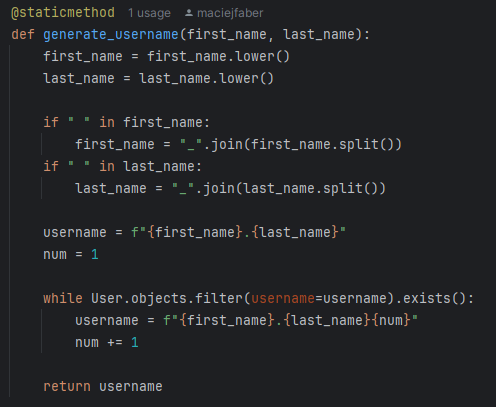
\includegraphics[width=0.8\textwidth]{images/krzysztofBImages/genrate_usernama.png}
    \caption{funkcja generująca unikalne nazwy użytkownika.}
    \emph{Źródło: opracowanie własne.}
    \label{fig:username_generation}
\end{figure}
\begin{figure}[H]
    \centering
    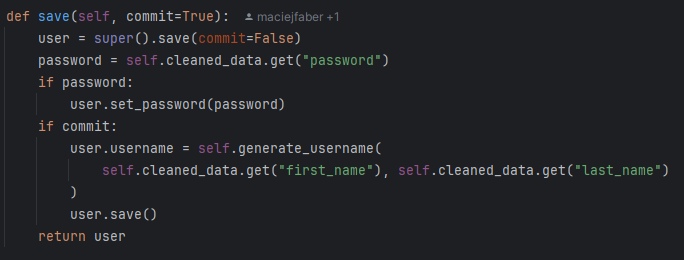
\includegraphics[width=0.8\textwidth]{images/krzysztofBImages/register_save.png}
    \caption{Metoda save używająca funkcji \texttt{generate\_username}.}
    \emph{Źródło: opracowanie własne.}
    \label{fig:username_generation_use}
\end{figure}
%
%
\subsubsection{Maciej Faber: Widok logowania umożliwiający logowanie przy użyciu adresu e-mail}
\label{section:1.3.38}
\textit{
Implementacja widoku logowania, który umożliwia uwierzytelnianie użytkowników za pomocą adresu e-mail zamiast nazwy użytkownika.
}
Zaimplementowano następujące elementy:
\begin{itemize}
    \item \textbf{Dostosowanie formularza logowania:}
    \begin{itemize}
        \item Formularz przyjmuje adres e-mail jako dane uwierzytelniające.
        \item Walidacja adresu e-mail w celu zapewnienia poprawności danych wejściowych.
    \end{itemize}
    \begin{figure}[H]
        \centering
        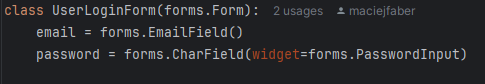
\includegraphics[width=0.8\textwidth]{images/krzysztofBImages/login_form_view.png}
        \caption{Formularz logowania z obsługą adresu e-mail.}
        \emph{Źródło: opracowanie własne.}
        \label{fig:email_login_form}
    \end{figure}
    \item \textbf{Modyfikacja mechanizmu uwierzytelniania:}
    \begin{itemize}
        \item Zmiana algorytmu logowania, aby wyszukiwał użytkowników na podstawie adresu e-mail.
        \item Obsługa błędów uwierzytelnienia, takich jak nieprawidłowe hasło lub brak konta powiązanego z podanym adresem e-mail.
    \end{itemize}
\end{itemize}
\begin{figure}[H]
    \centering
    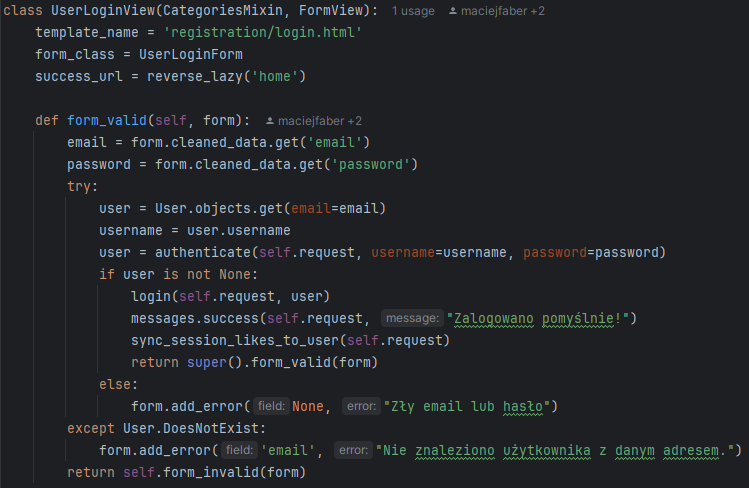
\includegraphics[width=0.8\textwidth]{images/krzysztofBImages/login_view.png}
    \caption{Widok logowania z obsługą adresu e-mail.}
    \emph{Źródło: opracowanie własne.}
    \label{fig:email_login}
\end{figure}
%
%
\subsubsection{Maciej Faber: Modele \texttt{Cart} i \texttt{CartItem} oraz widok dodawania produktów do koszyka}
\label{section:1.3.39}
\textit{
Implementacja modeli \texttt{Cart} i \texttt{CartItem} w celu obsługi koszyka zakupowego oraz widoku umożliwiającego dodawanie produktów do koszyka.
}
Zaimplementowano następujące elementy:
\begin{itemize}
    \item \textbf{Model \texttt{Cart}:}
    \begin{itemize}
        \item Reprezentuje koszyk użytkownika, powiązany z użytkownikiem (lub anonimowy).
        \item Przechowuje datę utworzenia i ostatniej aktualizacji.
        \item Zawiera metodę \texttt{get\_total\_price}, która oblicza łączną cenę produktów w koszyku.
    \end{itemize}
    \item \textbf{Model \texttt{CartItem}:}
    \begin{itemize}
        \item Przechowuje informacje o produkcie, ilości i koszyku, do którego należy.
        \item Zawiera metodę \texttt{get\_total\_price}, która oblicza cenę dla danego produktu na podstawie ilości.
    \end{itemize}
    \begin{figure}[H]
        \centering
        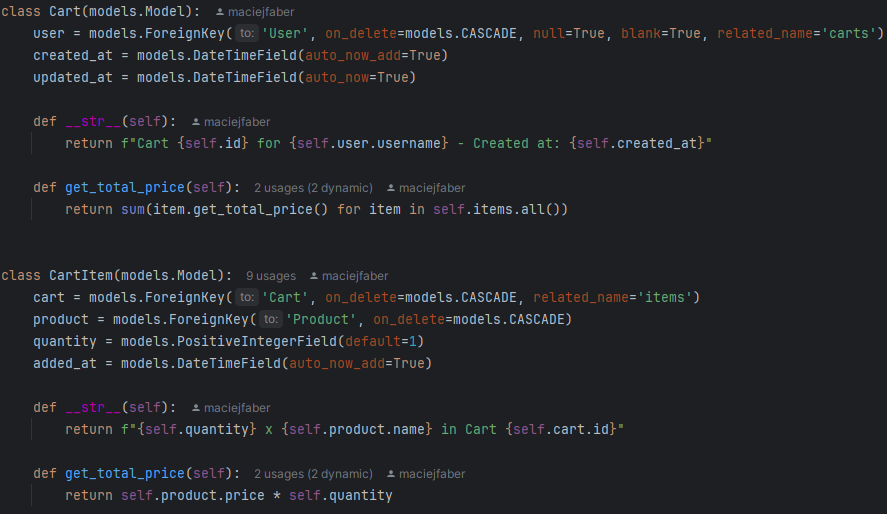
\includegraphics[width=0.8\textwidth]{images/krzysztofBImages/cart_models.png}
        \caption{Modele obsługujące koszyk zakupowy.}
        \label{fig:cart_models}
    \end{figure}
    \item \textbf{Widok \texttt{AddToCartView}:}
    \begin{itemize}
        \item Obsługuje dodawanie produktów do koszyka z możliwością ustawienia ilości.
        \item Obsługuje zarówno użytkowników zalogowanych, jak i anonimowych,\\ przechowując koszyk w sesji.
        \item Obsługuje żądania asynchroniczne (AJAX) i zwraca odpowiedni JSON w przypadku sukcesu.
    \end{itemize}
    \item \textbf{Integracja z panelem administratora:}
    \begin{itemize}
        \item Modele \texttt{Cart} i \texttt{CartItem} zostały zarejestrowane w panelu administratora, umożliwiając ich przeglądanie i edycję.
    \end{itemize}
\end{itemize}
\begin{figure}[H]
    \centering
    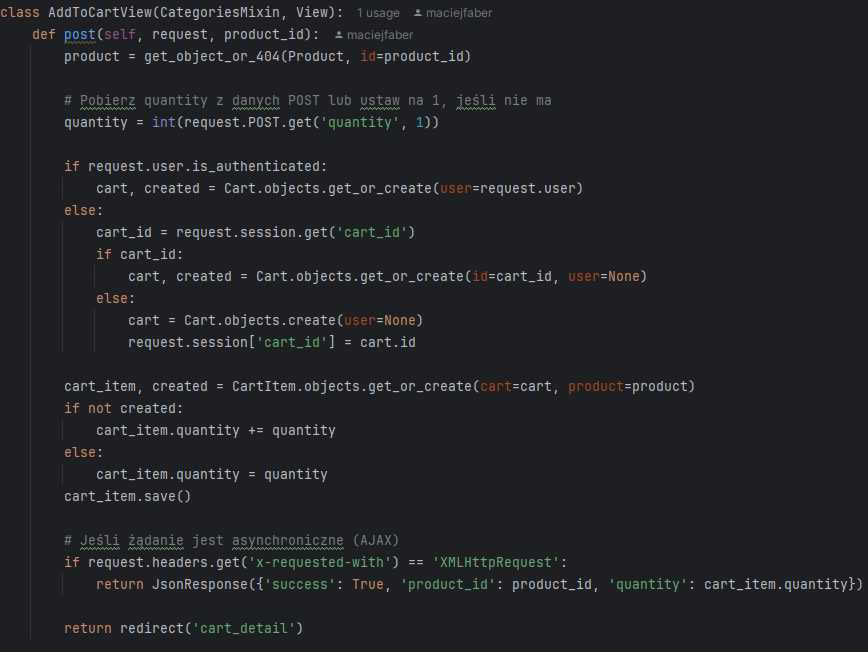
\includegraphics[width=0.8\textwidth]{images/krzysztofBImages/add_to_cart_view.png}
    \caption{Widok dodawania produktu do koszyka.}
    \emph{Źródło: opracowanie własne.}
    \label{fig:add_to_cart}
\end{figure}
%
%
\subsubsection{Maciej Faber: Widoki obsługujące usuwanie oraz modyfikację ilości produktów w koszyku}
\label{section:1.3.40}
\textit{
Implementacja widoków umożliwiających usunięcie produktu z koszyka oraz modyfikację ilości produktów w koszyku.
}
Zaimplementowano następujące elementy:
\begin{itemize}
    \item \textbf{Widok \texttt{RemoveFromCartView}:}
    \begin{itemize}
        \item Obsługuje usuwanie produktów z koszyka.
        \item Obsługuje zarówno użytkowników zalogowanych, jak i anonimowych,\\ umożliwiając usuwanie produktów na podstawie sesji lub użytkownika.
        \item Zwraca odpowiedź JSON w przypadku żądań asynchronicznych (AJAX).
    \end{itemize}
    \begin{figure}[H]
        \centering
        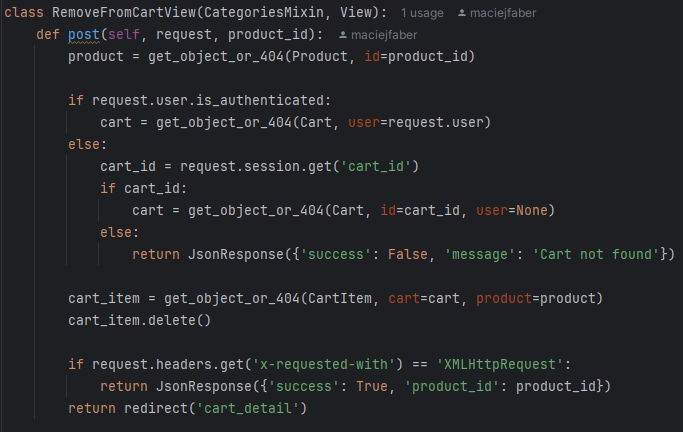
\includegraphics[width=0.8\textwidth]{images/krzysztofBImages/remove_from_cart_view.png}
        \caption{Widok usuwający produkt z koszyka.}
        \emph{Źródło: opracowanie własne.}
        \label{fig:remove_item_cart}
    \end{figure}
    \item \textbf{Widok \texttt{UpdateCartItemView}:}
    \begin{itemize}
        \item Obsługuje zwiększanie i zmniejszanie ilości produktów w koszyku.
        \item Akceptuje akcje \texttt{increase}, \texttt{decrease} oraz wartość ilości podaną w parametrze \texttt{quantity}.
        \item Weryfikuje poprawność wprowadzonych danych oraz obsługuje błędy, takie jak ilość mniejsza od 1.
        \item Zwraca odpowiedź JSON w przypadku żądań asynchronicznych (AJAX).
    \end{itemize}
\end{itemize}
\begin{figure}[H]
    \centering
    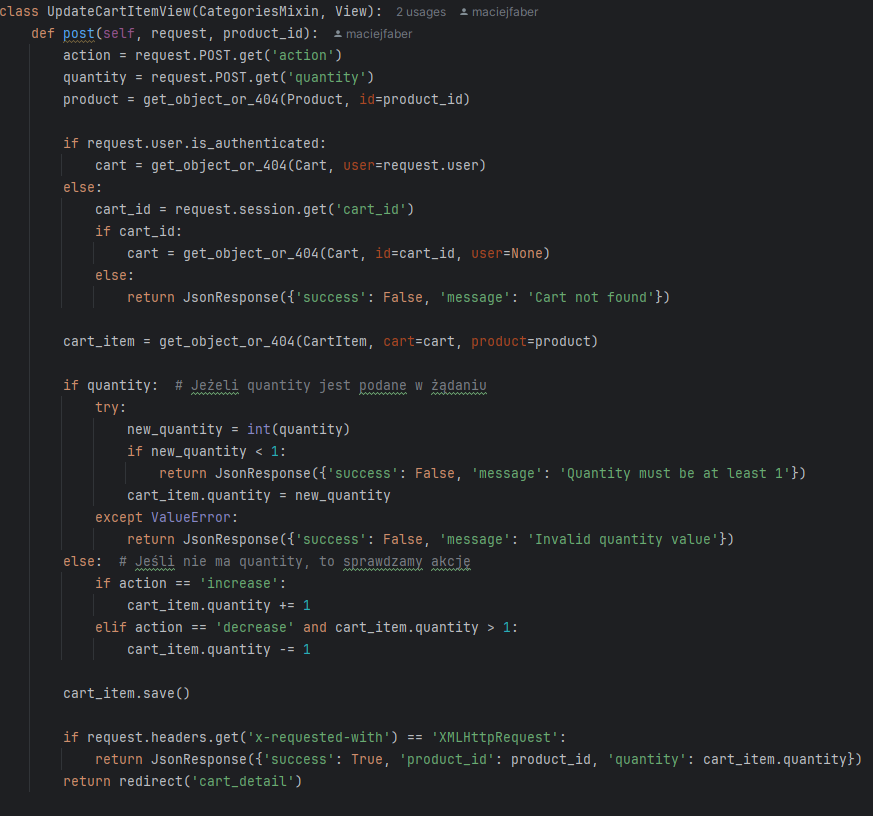
\includegraphics[width=0.8\textwidth]{images/krzysztofBImages/update_cart_item_view.png}
    \caption{Widok modyfikacji ilości produktów w koszyku.}
    \emph{Źródło: opracowanie własne.}
    \label{fig:update_cart}
\end{figure}
%
%
\subsubsection{Maciej Faber: Konfiguracja i obsługa wysyłania e-maili za pomocą Gmail API}
\label{section:1.3.41}
\textit{
Integracja aplikacji z usługą Gmail poprzez Gmail API w celu umożliwienia wysyłania e-maili, takich jak powiadomienia o rejestracji użytkowników.
}
Zaimplementowano następujące elementy:
\begin{itemize}
    \item \textbf{Konfiguracja Gmail API:}
    \begin{itemize}
        \item Utworzenie konta e-mail w usłudze Gmail i włączenie Gmail API w konsoli deweloperskiej Google.
        \item Pobranie danych uwierzytelniających (plik \texttt{email\_settings.py}) i ich integracja z aplikacją.
    \end{itemize}
    \item \textbf{Funkcja wysyłająca e-maile:}
    \begin{itemize}
        \item Implementacja funkcji umożliwiającej wysyłanie wiadomości e-mail do użytkowników.
        \item Powiadomienia o rejestracji użytkownika, w tym dynamiczne dostosowywanie treści e-maila na podstawie danych użytkownika.
    \end{itemize}
\end{itemize}
\begin{figure}[H]
    \centering
    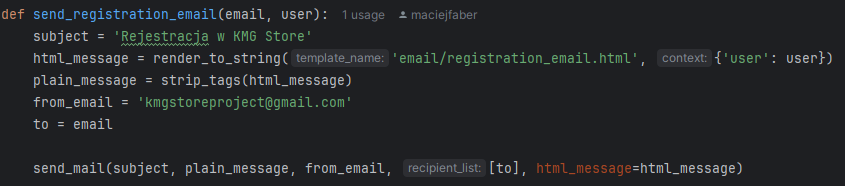
\includegraphics[width=0.8\textwidth]{images/krzysztofBImages/send_email.png}
    \caption{Funkcja wysyłająca email z potiwerdzeniem rejestracji.}
    \emph{Źródło: opracowanie własne.}
    \label{fig:email_notification}
\end{figure}
%
%
\subsubsection{Maciej Faber: Import danych z pliku JSON do bazy danych aplikacji}
\label{section:1.3.42}
\textit{
Implementacja skryptu \texttt{import\_next\_json\_to\_database.py}, który importuje dane z pliku \texttt{products\_seeded\_data.json} do bazy danych aplikacji.
}
Zaimplementowano następujące elementy:
\begin{itemize}
    \item \textbf{Obsługa pliku \texttt{products\_seeded\_data.json}:}
    \begin{itemize}
        \item Wczytanie danych z pliku JSON zawierającego informacje o produktach.
        \item Walidacja danych w celu zapewnienia ich spójności i kompletności.
    \end{itemize}
    \item \textbf{Przetwarzanie danych:}
    \begin{itemize}
        \item Implementacja funkcji \texttt{parse\_price} do przetwarzania cen\\ na format \texttt{Decimal}.
        \item Obsługa hierarchii kategorii za pomocą funkcji\\ \texttt{get\_or\_create\_category\_hierarchy}.
    \end{itemize}
    \item \textbf{Tworzenie obiektów w bazie danych:}
    \begin{itemize}
        \item Automatyczne tworzenie produktów w bazie danych na podstawie danych JSON.
        \item Przypisywanie kategorii do produktów oraz obsługa relacji między nimi.
    \end{itemize}
    \item \textbf{Logowanie i debugowanie:}
    \begin{itemize}
        \item Wyświetlanie komunikatów w konsoli dla każdego utworzonego produktu.
        \item Informowanie o ewentualnych błędach podczas importu.
    \end{itemize}
\end{itemize}
\begin{figure}[H]
    \centering
    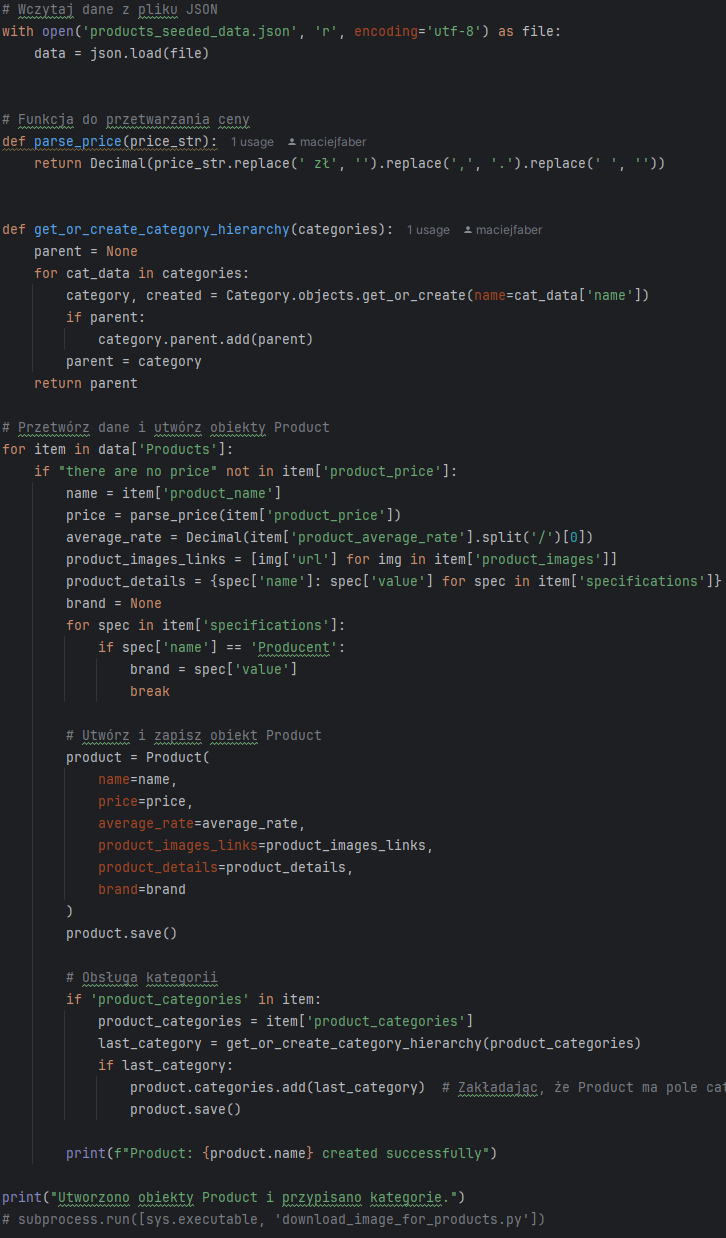
\includegraphics[width=0.8\textwidth]{images/krzysztofBImages/product_seed_to_database.png}
    \caption{Program przetwarzający dane z pliku JSON do bazy danych.}
    \emph{Źródło: opracowanie własne.}
    \label{fig:json_import}
\end{figure}
%
%
\subsubsection{Maciej Faber: Pobieranie zdjęć produktów z linków i zapisywanie ich w aplikacji}
\label{section:1.3.43}
\textit{
Implementacja skryptu pobierającego zdjęcia dla produktów na podstawie linków zapisanych w modelu \texttt{Product} w polu \texttt{product\_images\_links}.
}
Zaimplementowano następujące elementy:
\begin{itemize}
    \item \textbf{Funkcja \texttt{download\_image}:}
    \begin{itemize}
        \item Obsługuje pobieranie obrazów z podanych linków za pomocą\\ żądań HTTP.
        \item Zabezpieczenie przed błędami poprzez obsługę wyjątków i logowanie błędów.
    \end{itemize}
    \item \textbf{Funkcja \texttt{save\_product\_image}:}
    \begin{itemize}
        \item Tworzy tymczasowy plik obrazu na podstawie pobranych danych.
        \item Przypisuje obraz do produktu, zapisując go w systemie plików aplikacji.
    \end{itemize}
    \item \textbf{Obsługa brakujących lub niepoprawnych danych:}
    \begin{itemize}
        \item W przypadku braku linków ustawiany jest domyślny\\ obraz \texttt{default\_product.png}.
        \item Informowanie użytkownika o sukcesie lub błędach w procesie za pomocą komunikatów w konsoli.
    \end{itemize}
    \item \textbf{Iteracja po produktach:}
    \begin{itemize}
        \item Automatyczne przetwarzanie wszystkich produktów zapisanych w bazie danych.
        \item Pobieranie pierwszego dostępnego linku z listy \texttt{product\_images\_links} i ustawienie go jako główna grafika produktu.
    \end{itemize}
\end{itemize}
\begin{figure}[H]
    \centering
    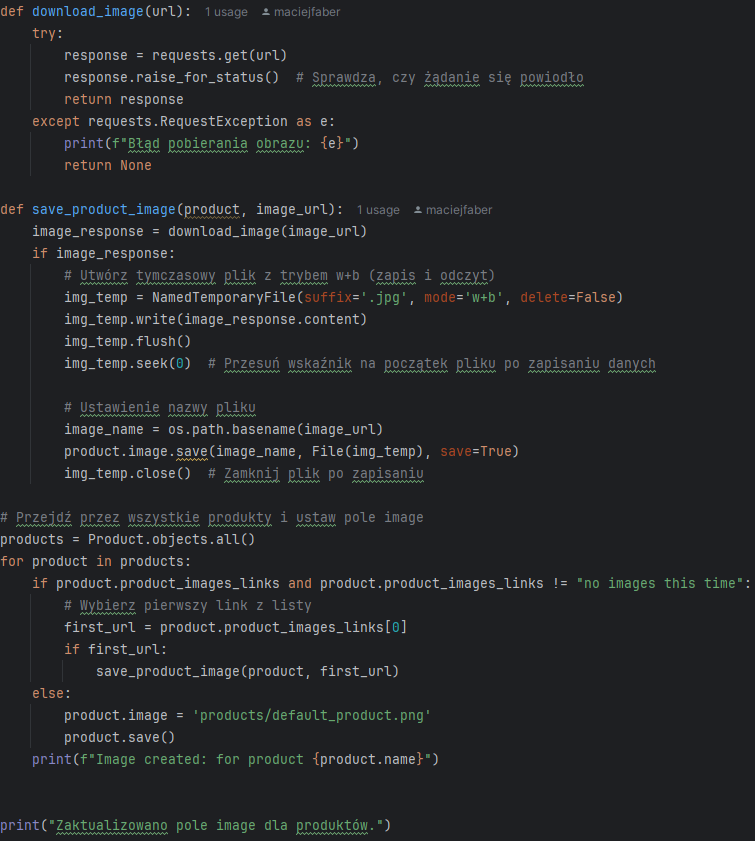
\includegraphics[width=0.8\textwidth]{images/krzysztofBImages/image_import.png}
    \caption{Funkcja służąca do pobierania zdjęcia dla produktu.}
    \emph{Źródło: opracowanie własne.}
    \label{fig:image_download}
\end{figure}
%
%
\subsubsection{Maciej Faber: Sortowanie wyświetlanych produktów}
\label{section:1.3.44}
\textit{
Dodanie możliwości sortowania produktów według różnych kryteriów.
}
Zaimplementowano następujące elementy:
\begin{itemize}
    \item \textbf{Sortowanie według ceny:}
    \begin{itemize}
        \item Rosnąco według ceny (\texttt{price\_asc}).
        \item Malejąco według ceny (\texttt{price\_desc}).
    \end{itemize}
    \item \textbf{Sortowanie według oceny:}
    \begin{itemize}
        \item Rosnąco według średniej oceny (\texttt{rating\_asc}).
        \item Malejąco według średniej oceny (\texttt{rating\_desc}).
    \end{itemize}
    \item \textbf{Sortowanie według popularności:}
    \begin{itemize}
        \item Rosnąco według liczby polubień (\texttt{popularity\_asc}).
        \item Malejąco według liczby polubień (\texttt{popularity\_desc}).
    \end{itemize}
    \item \textbf{Mechanizm implementacji:}
    \begin{itemize}
        \item Pobieranie wartości parametru \texttt{sort\_by} z zapytania GET.
        \item Dynamiczne sortowanie wyników na podstawie podanej wartości.
    \end{itemize}
\end{itemize}
\begin{figure}[H]
    \centering
    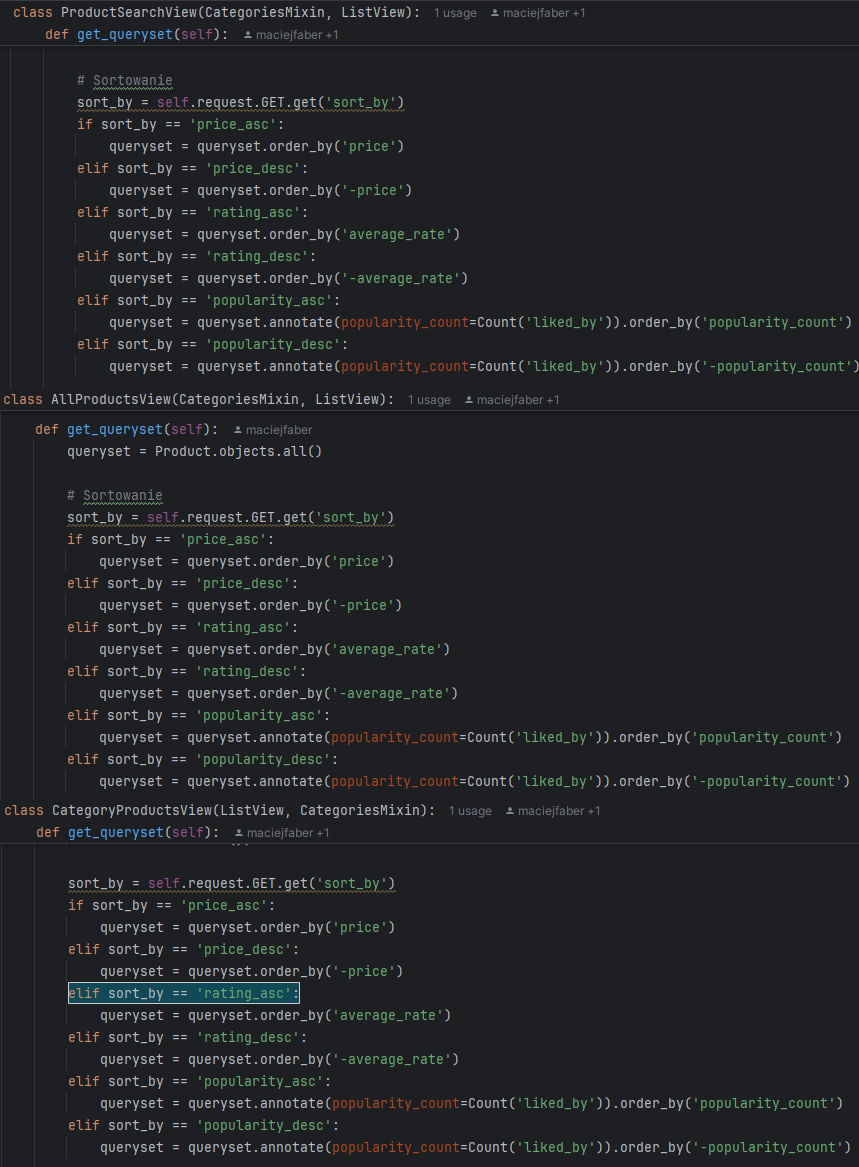
\includegraphics[width=0.8\textwidth]{images/krzysztofBImages/sorting.png}
    \caption{Implementacja kodu sortowania produktów.}
    \emph{Źródło: opracowanie własne.}
    \label{fig:sorting_products}
\end{figure}
%
%
\subsubsection{Maciej Faber: Filtrowanie wyświetlanych produktów}
\label{section:1.3.45}
\textit{
Dodanie możliwości filtrowania produktów według zakresu cen.
}
Zaimplementowano następujące elementy:
\begin{itemize}
    \item \textbf{Filtrowanie według ceny:}
    \begin{itemize}
        \item Minimalna cena produktu (parametr \texttt{min\_price}).
        \item Maksymalna cena produktu (parametr \texttt{max\_price}).
    \end{itemize}
    \item \textbf{Mechanizm implementacji:}
    \begin{itemize}
        \item Pobieranie wartości parametrów \texttt{min\_price} i \texttt{max\_price}\\ z zapytania GET.
        \item Dynamiczne filtrowanie wyników w zależności od podanego zakresu cen.
    \end{itemize}
    \item \textbf{Obsługa błędnych wartości:}
    \begin{itemize}
        \item Ignorowanie parametrów, jeśli ich wartości są puste lub nieprawidłowe.
    \end{itemize}
\end{itemize}
\begin{figure}[H]
    \centering
    \includegraphics[width=0.8\textwidth]{images/krzysztofBImages/filter_price.png}
    \caption{Implementacja kodu filtrowania produktów według zakresu cen.}
    \emph{Źródło: opracowanie własne.}
    \label{fig:filtering_products}
\end{figure}
\subsection{Załączniki}
\textit{Lista załączników lub dodatkowych materiałów potwierdzających zrealizowane zadania.}
%
%
\subsubsection{Maciej Faber: Dodanie kodu HTML obsługującego sortowanie w szablonach}
\label{section:1.3.46}
\textit{
Dodanie kodu HTML umożliwiającego obsługę sortowania produktów w interfejsie użytkownika.
}
Zaimplementowano następujące elementy:
\begin{itemize}
    \item \textbf{Element interfejsu użytkownika:}
    \begin{itemize}
        \item Przyciski rozwijanego menu umożliwiające wybór kryteriów sortowania.
        \item Opcje sortowania obejmujące:
        \begin{itemize}
            \item Sortowanie domyślne.
            \item Cena: rosnąco i malejąco.
            \item Ocena: rosnąco i malejąco.
            \item Popularność: rosnąco i malejąco.
        \end{itemize}
    \end{itemize}
    \item \textbf{Obsługa parametrów w linkach:}
    \begin{itemize}
        \item Dynamiczne wstawianie wartości \texttt{min\_price} i \texttt{max\_price} do linków w celu zachowania aktualnych filtrów.
        \item Wykorzystanie parametru \texttt{sort\_by} w adresie URL.
    \end{itemize}
    \item \textbf{Integracja z backendem:}
    \begin{itemize}
        \item Przekazywanie parametrów sortowania do widoków za pomocą zapytań GET.
        \item Wyświetlanie aktualnego kryterium sortowania w przycisku rozwijanego menu.
    \end{itemize}
\end{itemize}
\begin{figure}[H]
    \centering
    \includegraphics[width=0.8\textwidth]{images/krzysztofBImages/html_sorting.png}
    \caption{Interfejs użytkownika z obsługą sortowania produktów.}
    \emph{Źródło: opracowanie własne.}
    \label{fig:sorting_html}
\end{figure}
%
%
\subsubsection{Maciej Faber: Model \texttt{UserProductVisibility} i logowanie wyświetlanych produktów}
\label{section:1.3.47}
\textit{
Implementacja modelu \texttt{UserProductVisibility} i wykorzystanie go do rejestrowania wyświetleń produktów przez użytkowników.
}
Zaimplementowano następujące elementy:
\begin{itemize}
    \item \textbf{Model \texttt{UserProductVisibility}:}
    \begin{itemize}
        \item Powiązanie użytkownika z produktem oraz zapis daty wyświetlenia.
        \item Automatyczne dodanie wpisu przy każdym wyświetleniu produktu.
    \end{itemize}
    \begin{figure}[H]
        \centering
        \includegraphics[width=0.8\textwidth]{images/krzysztofBImages/product_visibility_model.png}
        \caption{Model \texttt{UserProductVisibility}.}
        \emph{Źródło: opracowanie własne.}
        \label{fig:user_product_visibility_model}
    \end{figure}
    \item \textbf{Mechanizm logowania wyświetleń:}
    \begin{itemize}
        \item Dla zalogowanych użytkowników:
        \begin{itemize}
            \item Tworzenie wpisu w bazie danych tylko wtedy, gdy produkt nie był wyświetlany w ciągu ostatniej godziny.
        \end{itemize}
        \item Dla użytkowników anonimowych:
        \begin{itemize}
            \item Przechowywanie informacji o wyświetleniach w sesji.
            \item Sprawdzanie, czy produkt nie był wyświetlany w ciągu ostatniej godziny.
        \end{itemize}
    \end{itemize}
    \item \textbf{Integracja z widokiem produktu:}
    \begin{itemize}
        \item Rejestracja wyświetlenia produktu przy każdym zapytaniu GET do widoku produktu.
        \item Obsługa zarówno użytkowników zalogowanych, jak i anonimowych.
    \end{itemize}
\end{itemize}
\begin{figure}[H]
    \centering
    \includegraphics[width=0.8\textwidth]{images/krzysztofBImages/product_visibility_usage.png}
    \caption{Model \texttt{UserProductVisibility} w widoku produktu.}
    \emph{Źródło: opracowanie własne.}
    \label{fig:user_product_visibility}
\end{figure}
%
%
\subsubsection{Maciej Faber: Model \texttt{UserCategoryVisibility} i logowanie wyświetlanych kategorii}
\label{section:1.3.48}
\textit{
Implementacja modelu \texttt{UserCategoryVisibility} i wykorzystanie go do rejestrowania wyświetleń kategorii przez użytkowników.
}
Zaimplementowano następujące elementy:
\begin{itemize}
    \item \textbf{Model \texttt{UserCategoryVisibility}:}
    \begin{itemize}
        \item Powiązanie użytkownika z kategorią oraz zapis daty wyświetlenia.
        \item Automatyczne dodanie wpisu przy każdym wyświetleniu kategorii.
    \end{itemize}
    \begin{figure}[H]
        \centering
        \includegraphics[width=0.8\textwidth]{images/krzysztofBImages/category_visibility_model.png}
        \caption{Model \texttt{UserCategoryVisibility}.}
        \emph{Źródło: opracowanie własne.}
        \label{fig:user_category_visibility_model}
    \end{figure}
    \item \textbf{Mechanizm logowania wyświetleń:}
    \begin{itemize}
        \item Dla zalogowanych użytkowników:
        \begin{itemize}
            \item Tworzenie wpisu w bazie danych tylko wtedy, gdy kategoria nie była wyświetlana w ciągu ostatniej godziny.
        \end{itemize}
        \item Dla użytkowników anonimowych:
        \begin{itemize}
            \item Przechowywanie informacji o wyświetleniach w sesji.
            \item Sprawdzanie, czy kategoria nie była wyświetlana w ciągu ostatniej godziny.
        \end{itemize}
    \end{itemize}
    \item \textbf{Integracja z widokiem kategorii:}
    \begin{itemize}
        \item Rejestracja wyświetlenia kategorii przy każdym zapytaniu GET do widoku kategorii.
        \item Obsługa zarówno użytkowników zalogowanych, jak i anonimowych.
    \end{itemize}
\end{itemize}
\begin{figure}[H]
    \centering
    \includegraphics[width=0.8\textwidth]{images/krzysztofBImages/category_visibility_usage.png}
    \caption{Model \texttt{UserCategoryVisibility} w widoku.}
    \emph{Źródło: opracowanie własne.}
    \label{fig:user_category_visibility}
\end{figure}
%
%
\subsubsection{Maciej Faber: Model \texttt{UserQueryLog} i logowanie zapytań użytkownika}
\label{section:1.3.49}
\textit{
Implementacja modelu \texttt{UserQueryLog} do rejestrowania zapytań wyszukiwania wprowadzanych przez użytkowników.
}
Zaimplementowano następujące elementy:
\begin{itemize}
    \item \textbf{Model \texttt{UserQueryLog}:}
    \begin{itemize}
        \item Powiązanie użytkownika z zapytaniem i zapis daty wykonania zapytania.
        \item Przechowywanie treści zapytania w bazie danych.
    \end{itemize}
    \begin{figure}[H]
        \centering
        \includegraphics[width=0.8\textwidth]{images/krzysztofBImages/query_log_model.png}
        \caption{Model \texttt{UserQueryLog}.}
        \emph{Źródło: opracowanie własne.}
        \label{fig:user_query_log_model}
    \end{figure}
    \item \textbf{Mechanizm logowania zapytań:}
    \begin{itemize}
        \item Dodawanie wpisu do bazy danych dla każdego zapytania wprowadzonego przez użytkownika.
        \item Możliwość analizy historii wyszukiwań użytkownika.
    \end{itemize}
\end{itemize}
\begin{figure}[H]
    \centering
    \includegraphics[width=0.8\textwidth]{images/krzysztofBImages/query_log_usage.png}
    \caption{Model \texttt{UserQueryLog} w widoku.}
    \emph{Źródło: opracowanie własne.}
    \label{fig:user_query_log}
\end{figure}
%
%
\subsubsection{Maciej Faber: Modele używane w algorytmie rekomendacyjnym}
\label{section:1.3.50}
\textit{
Implementacja modeli \texttt{RecommendedProducts} oraz \texttt{UserRecommendedProductInteraction}, które wspierają działanie algorytmu rekomendacyjnego.
}
Zaimplementowano następujące elementy:
\begin{itemize}
    \item \textbf{Model \texttt{RecommendedProducts}:}
    \begin{itemize}
        \item Powiązanie użytkownika z listą rekomendowanych produktów.
        \item Przechowywanie wielu produktów przypisanych do użytkownika.
        \item Automatyczne dodanie daty wygenerowania rekomendacji.
    \end{itemize}
    \item \textbf{Model \texttt{UserRecommendedProductInteraction}:}
    \begin{itemize}
        \item Zapis interakcji użytkownika z rekomendowanymi produktami.
        \item Typy interakcji obejmujące:
        \begin{itemize}
            \item \texttt{view} - wyświetlenie produktu,
            \item \texttt{like} - polubienie produktu,
            \item \texttt{buy} - zakup produktu.
        \end{itemize}
        \item Automatyczne dodanie daty interakcji.
    \end{itemize}
    \item \textbf{Przydatność dla algorytmu rekomendacyjnego:}
    \begin{itemize}
        \item Analiza zachowań użytkowników na podstawie interakcji.
        \item Wykorzystanie zapisanych interakcji do dostosowania rekomendacji w czasie rzeczywistym.
    \end{itemize}
\end{itemize}
\begin{figure}[H]
    \centering
    \includegraphics[width=0.8\textwidth]{images/krzysztofBImages/recomended_models.png}
    \caption{Modele rekomendacji produktów.}
    \emph{Źródło: opracowanie własne.}
    \label{fig:recommended_products}
\end{figure}
%
%
\subsubsection{Maciej Faber: Funkcje algorytmu rekomendacyjnego — wyszukiwanie podobnych produktów}
\label{section:1.3.51}
\textit{
Implementacja funkcji do wyszukiwania podobnych produktów oraz początkowych etapów algorytmu rekomendacyjnego.
}
Zaimplementowano następujące elementy:
\begin{itemize}
    \item \textbf{Funkcja \texttt{get\_similar\_products}:}
    \begin{itemize}
        \item Znajdowanie produktów podobnych na podstawie kategorii.
        \item Analiza słów kluczowych w nazwie produktu.
        \item Scalanie wyników i eliminacja duplikatów.
    \end{itemize}
    \item \textbf{Funkcja \texttt{get\_recommended\_products}:}
    \begin{itemize}
        \item Wprowadzenie wagi punktacji dla różnych interakcji użytkownika z produktami.
        \item Analiza kategorii wyświetlanych przez użytkownika.
        \item Uwzględnienie zakupów użytkownika oraz podobnych produktów.
        \item Obsługa błędów za pomocą \texttt{try-except} dla wyjątków związanych z modelem \texttt{RecommendedProducts}.
    \end{itemize}
\end{itemize}
\begin{figure}[H]
    \centering
    \includegraphics[width=0.8\textwidth]{images/krzysztofBImages/recommended_algorithm_1.png}
    \caption{Proces wyszukiwania podobnych produktów wraz z algorytmem rekomendacyjnym.}
    \emph{Źródło: opracowanie własne.}
    \label{fig:recommendation_step1}
\end{figure}
\begin{figure}[H]
    \centering
    \includegraphics[width=0.8\textwidth]{images/krzysztofBImages/recommended_algorithm_2.png}
    \caption{Algorytm rekomendacyjny cz.2.}
    \emph{Źródło: opracowanie własne.}
    \label{fig:recommendation_step2}
\end{figure}

\subsubsection{Maciej Faber: Punktacja za interakcje z rekomendowanymi produktami}
\label{section:1.3.52}
\textit{
Rozszerzenie algorytmu rekomendacyjnego o punktację za interakcje użytkownika z wcześniej rekomendowanymi produktami.
}
Zaimplementowano następujące elementy:
\begin{itemize}
    \item \textbf{Uwzględnienie interakcji użytkownika z rekomendacjami:}
    \begin{itemize}
        \item Dodanie punktacji za produkty wyświetlone po rekomendacji.
        \item Uwzględnienie podobnych produktów wyświetlonych, polubionych lub zakupionych po rekomendacji.
    \end{itemize}
    \item \textbf{Rejestrowanie interakcji użytkownika:}
    \begin{itemize}
        \item Tworzenie wpisów w modelu \texttt{UserRecommendedProductInteraction} dla wyświetleń, polubień i zakupów.
        \item Integracja rejestrowania z algorytmem rekomendacyjnym.
    \end{itemize}
    \item \textbf{Zapis i sortowanie rekomendacji:}
    \begin{itemize}
        \item Sortowanie produktów według punktacji.
        \item Zapisanie listy rekomendacji w modelu \texttt{RecommendedProducts}.
        \item Obsługa przypadku, gdy lista rekomendacji jest pusta — losowe produkty.
    \end{itemize}
\end{itemize}
\begin{figure}[H]
    \centering
    \includegraphics[width=0.8\textwidth]{images/krzysztofBImages/recommended_algorithm_update.png}
    \caption{Punktacja za interakcje z rekomendacjami.}
    \emph{Źródło: opracowanie własne.}
    \label{fig:recommendation_step3}
\end{figure}
%
%
\subsubsection{Maciej Faber: Algorytm rekomendacyjny dla sesji}
\label{section:1.3.53}
\textit{
Implementacja algorytmu rekomendacyjnego działającego na podstawie danych przechowywanych w sesji użytkownika.
}
Zaimplementowano następujące elementy:
\begin{itemize}
    \item \textbf{Analiza danych z sesji:}
    \begin{itemize}
        \item Wykorzystanie polubionych produktów, wyświetlonych produktów oraz zapytań z sesji.
        \item Punktacja za widoczność kategorii produktów w sesji.
    \end{itemize}
    \item \textbf{Interakcje innych użytkowników:}
    \begin{itemize}
        \item Uwzględnienie produktów polubionych przez innych użytkowników.
        \item Dodanie produktów kupionych przez użytkowników o podobnych polubieniach.
    \end{itemize}
    \item \textbf{Generowanie rekomendacji:}
    \begin{itemize}
        \item Sortowanie produktów według punktacji.
        \item Filtrowanie produktów, które użytkownik już polubił w sesji.
        \item Obsługa przypadku pustej listy rekomendacji poprzez losowanie produktów.
    \end{itemize}
\end{itemize}
\begin{figure}[H]
    \centering
    \includegraphics[width=0.8\textwidth]{images/krzysztofBImages/session_recommendations.png}
    \caption{Algorytm rekomendacyjny dla sesji.}
    \emph{Źródło: opracowanie własne.}
    \label{fig:session_recommendations}
\end{figure}
%
%
\subsubsection{Maciej Faber: Program do skalowania zdjęć produktów}
\label{section:1.3.54}
\textit{
Implementacja programu \texttt{resizer.py} do skalowania zdjęć produktów w celu wyeliminowania problemów ze skalowaniem w interfejsie użytkownika.
}
Zaimplementowano następujące elementy:
\begin{itemize}
    \item \textbf{Funkcja \texttt{resize\_images\_with\_proportions}:}
    \begin{itemize}
        \item Skalowanie zdjęć z zachowaniem proporcji oryginalnych obrazów.
        \item Tworzenie białego tła dla zdjęć o nieregularnych proporcjach, aby dopasować je do wymaganego rozmiaru.
    \end{itemize}
    \item \textbf{Proces skalowania:}
    \begin{itemize}
        \item Skalowanie zdjęć w formatach JPG i PNG do rozmiaru \texttt{1064x1064 px}.
        \item Zapisanie przetworzonych zdjęć w oryginalnym katalogu z zachowaniem ich nazw.
    \end{itemize}
    \item \textbf{Zastosowanie w projekcie:}
    \begin{itemize}
        \item Wyeliminowanie problemów ze skalowaniem zdjęć produktów w interfejsie użytkownika.
        \item Usprawnienie wyświetlania produktów w spójny sposób w całej aplikacji.
    \end{itemize}
\end{itemize}
\begin{figure}[H]
    \centering
    \includegraphics[width=0.8\textwidth]{images/krzysztofBImages/resizer_image.png}
    \caption{Funkcja \texttt{resize\_images\_with\_proportions}}
    \emph{Źródło: opracowanie własne.}
    \label{fig:image_resizing}
\end{figure}

% --------------------------------------------------------------------
%%%%%%% odkomentować gdy bibliografia ma być wewnątrz dokumentu
% --------------------------------------------------------------------
%\begin{thebibliography}{11}
%
%\addcontentsline{toc}{section}{Literatura}
%
%\bibitem{ZAN}
%C. Zannoni and P. Pasini, 
%\emph{Advances in the Computer Simulatons of Liquid Crystals}, Kluwer Academic Publishers, 2000.
%
%\end{thebibliography}

\end{document}

